\documentclass[11pt,twoside]{report}
% PACKAGES
%\usepackage[bindingoffset=4cm]{geometry}
\usepackage{graphicx}
\usepackage[usenames,dvipsnames]{color}
\usepackage{booktabs}
\usepackage[colorlinks,linkcolor=black,pagebackref=true]{hyperref}
\usepackage[]{todonotes}
\usepackage[small, sf, bf]{caption}
\usepackage[utf8]{inputenc}
\usepackage{amsmath}
%\usepackage[toc,page]{appendix}
\usepackage{cleveref}
\usepackage{listings}
\usepackage{textcomp}
\usepackage{setspace}
\usepackage{palatino}
\usepackage[small,compact]{titlesec}
\usepackage[]{siunitx}
\usepackage{fancyhdr} % FANCY HEADERS
\usepackage{sectsty} % SECTION TITLES				
\usepackage[titles]{tocloft} % Control the fonts and formatting used in the table of contents.
\usepackage{subcaption}
\usepackage{nomencl}
\pagenumbering{roman}
\makenomenclature
\interfootnotelinepenalty=10000
\renewcommand{\bibname}{References}

% LINE SPACING
%\linespread{1.6}


% FANCY HEADERS

%E: Even page
%O: Odd page
%L: Left field
%C: Center field
%R: Right field
%H: Header
%F: Footer

\setlength{\headheight}{15pt}
 
\pagestyle{fancy}
\fancyhead{}
\fancyfoot{}

\renewcommand{\sectionmark}[1]{\markright{\thesection.\ #1}}
\lhead{\nouppercase{\rightmark}}
\rhead{\nouppercase{\leftmark}}

\renewcommand{\chaptermark}[1]{% 
\markboth{\chaptername 
\ \thechapter.\ #1}{}} 


%\fancyhead[RE,LO]{\slshape \rightmark}
\fancyhead[LE,RO] {\thepage}


% BRING WHITE SAPCE TO END OF PAGE
\raggedbottom


% CHEMICAL FORMULAS
\newcommand{\chem}[1]{\ensuremath{\mathrm{#1}}}

% PICTURE OFFSETS
\newlength{\PictHOffset}
\newlength{\PictVOffset}
\setlength{\PictHOffset}{0.8in}
\addtolength{\PictHOffset}{\hoffset}
\addtolength{\PictHOffset}{\oddsidemargin}

\setlength{\PictVOffset}{0.41in}
\addtolength{\PictVOffset}{\voffset}
\addtolength{\PictVOffset}{\topmargin}
\addtolength{\PictVOffset}{\headheight}
\addtolength{\PictVOffset}{\headsep}
\addtolength{\PictVOffset}{\topskip}
\addtolength{\PictVOffset}{-1\paperheight}

% SECTION TITLES
\sectionfont{\sffamily\selectfont}
\subsectionfont{\sffamily\selectfont}
\subsubsectionfont{\sffamily\selectfont}
\paragraphfont{\sffamily\selectfont}
%\setkomafont{sectioning}{\rmfamily\bfseries\boldmath}


% TOC SETTINGS
\setcounter{secnumdepth}{4}
\setcounter{tocdepth}{4}
%% Aesthetic spacing redefines that look nice
\setlength{\cftbeforechapskip}{4ex}
\setlength{\cftbeforesecskip}{0.6ex}
%% Use Helvetica-Narrow Bold for Chapter entries
\renewcommand{\cftchapfont}{\fontsize{11}{13}\usefont{OT1}{phv}{bc}{n}\selectfont}


% USER DEFINED COLORS
%\definecolor{deeppurple}{RGB}{77,0,255}
\definecolor{deeppurple}{RGB}{0,0,0} %well.. I made it black
\definecolor{deepblue}{RGB}{0,14,171}
\definecolor{bloody}{RGB}{144,21,0}
%\definecolor{titlecolourgold}{RGB}{250,250,210} 
\definecolor{titlecolourgold}{RGB}{230,230,230} %red
\definecolor{titlecolourpurple}{RGB}{138,43,226} 
\definecolor{titlecolourred}{RGB}{255,69,0}


% C CODE FORMATTING
\lstdefinestyle{my_C}
{ %
language=C,
basicstyle=\ttfamily\small\setstretch{1.1},
stringstyle=\color{black},
showstringspaces=false,
breaklines=false,                % sets automatic line breaking
alsoletter={1234567890},
otherkeywords={[1]\ , \}, \{},
keywordstyle=[1]\color{black}\bfseries,
emph={access,and,break,class,continue,def,del,elif ,else,%
except,exec,finally,for,from,global,if,import,in,i s,%
lambda,not,or,pass,print,raise,return,try,while,%
void,const,float,int},
emphstyle=\color{deeppurple}\bfseries,
%
emph={[2]from, import, as},
emphstyle=[2]\color{deeppurple}\bfseries,
upquote=true,
commentstyle=\color{black}\bfseries\slshape,
morecomment=[s][\color{bloody}]{"}{"},
morecomment=[s][\color{bloody}]{"""}{"""},
literate=*%{/}{{\bfseries{\textcolor{deeppurple}/}}}{1}%
{+}{{\bfseries{\textcolor{deeppurple}+}}}{1}%
{[}{{\bfseries{\textcolor{black}[}}}{1}%
{]}{{\bfseries{\textcolor{black}]}}}{1}%
{(}{{\bfseries{\textcolor{black}(}}}{1}%
{)}{{\bfseries{\textcolor{black})}}}{1}%
{=}{{\bfseries{\textcolor{black}=}}}{1}%
{-}{{\bfseries{\textcolor{deeppurple}-}}}{1}%
{*}{{\bfseries{\textcolor{deeppurple}*}}}{1},
numbers=none,                   % where to put the line-numbers
numberstyle=\footnotesize,      % the size of the fonts that are used for the line-numbers
stepnumber=1,
numbersep=5pt,                  % how far the line-numbers are from the code
backgroundcolor=\color{white},  % choose the background color. You must add \usepackage{color}
showspaces=false,               % show spaces adding particular underscores
showstringspaces=false,
showtabs=false,                 % show tabs within strings adding particular underscores
frame=leftline,	
tabsize=5,	                % sets default tabsize to 2 spaces
captionpos=t,                   % sets the caption-position to bottom
breakatwhitespace=false,        % sets if automatic breaks should only happen at whitespace
title=\lstname,  
linewidth= \textwidth,
xleftmargin= 0cm,
xrightmargin= 0cm,
frame=shadowbox,
frameround= tttt\thinlines
}



% PYTHON CODE FORMATTING
\lstdefinestyle{my_Python}
{ %
language=Python,
basicstyle=\ttfamily\small\setstretch{1},
stringstyle=\color{blue},
showstringspaces=false,
breaklines=true,                % sets automatic line breaking
alsoletter={1234567890},
otherkeywords={[1]\ , \}, \{},
keywordstyle=[1]\color{blue},
emph={access,and,break,class,continue,def,del,elif ,else,%
except,exec,finally,for,from,global,if,import,in,i s,%
lambda,not,or,pass,print,raise,return,try,while},
emphstyle=\color{deeppurple}\bfseries,
%
emph={[2]from, import, as},
emphstyle=[2]\color{deeppurple}\bfseries,
upquote=true,
commentstyle=\color{black}\bfseries\slshape,
morecomment=[s][\color{bloody}]{"}{"},
morecomment=[s][\color{bloody}]{"""}{"""},
literate=*{/}{{\bfseries{\textcolor{deeppurple}/}}}{1}%
{+}{{\bfseries{\textcolor{deeppurple}+}}}{1}%
{-}{{\bfseries{\textcolor{deeppurple}-}}}{1}%
{*}{{\bfseries{\textcolor{deeppurple}*}}}{1},
numbers=left,                   % where to put the line-numbers
numberstyle=\footnotesize,      % the size of the fonts that are used for the line-numbers
stepnumber=1,
numbersep=5pt,                  % how far the line-numbers are from the code
backgroundcolor=\color{white},  % choose the background color. You must add \usepackage{color}
showspaces=false,               % show spaces adding particular underscores
showstringspaces=false,
showtabs=false,                 % show tabs within strings adding particular underscores
frame=leftline,	
tabsize=3,	                % sets default tabsize to 2 spaces
captionpos=t,                   % sets the caption-position to bottom
breakatwhitespace=false,        % sets if automatic breaks should only happen at whitespace
title=\lstname,  
linewidth= 14cm,
xleftmargin= -2cm,
xrightmargin= 0cm 
}




\addtolength{\textwidth}{1cm}
\addtolength{\hoffset}{-0.5cm}
\addtolength{\textheight}{3cm}
\addtolength{\voffset}{-1.5cm}
%\oddsidemargin  0cm
%\evensidemargin 0cm


\begin{document}
% TITLE
\begin{titlepage}
   \noindent\hspace*{-\PictHOffset}%   
   \raisebox{\PictVOffset}[0pt][0pt]{\makebox[0pt][l]{%
      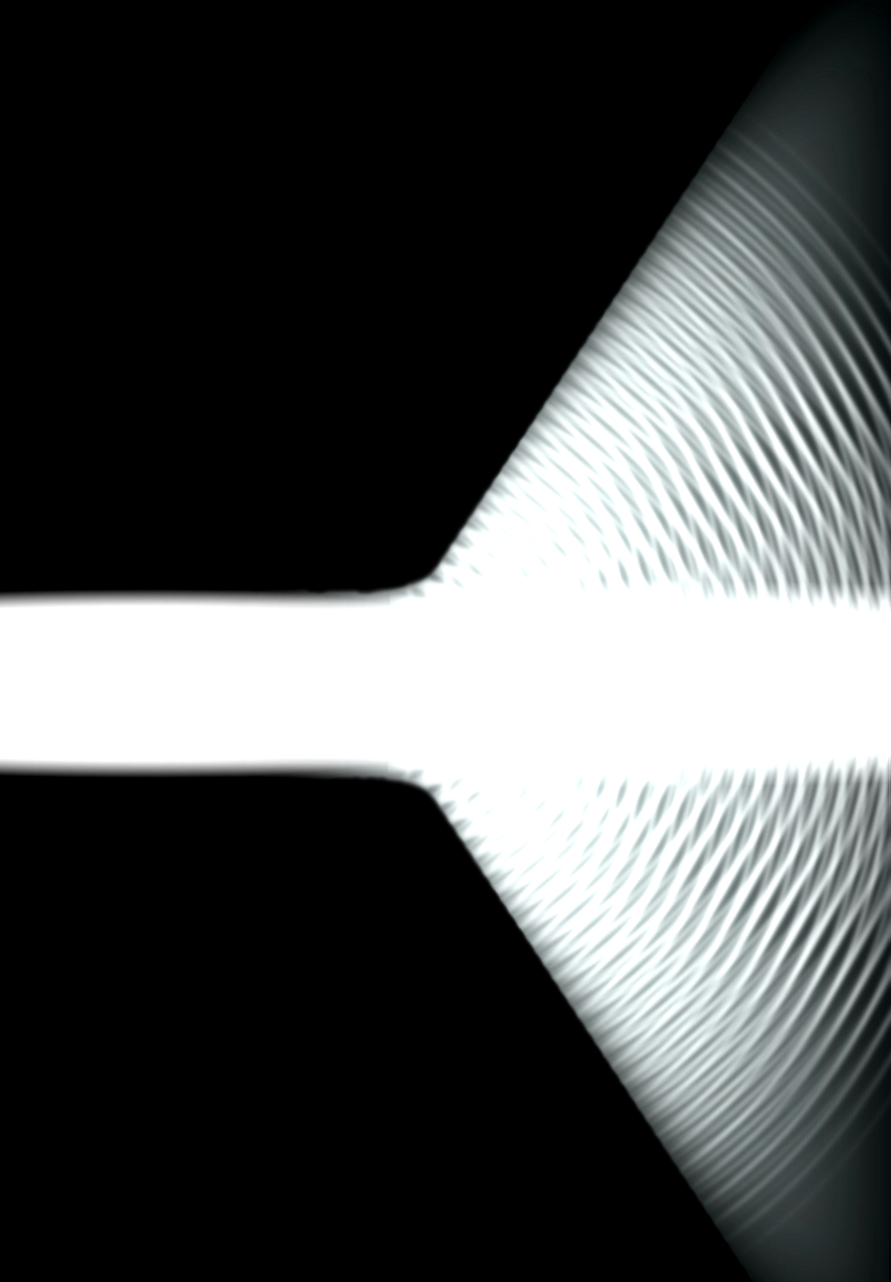
\includegraphics[width=\paperwidth,height=1.0\paperheight]{img/fp_v2_bright.png}}}
   
    %\raisebox{\PictVOffset}[0pt][0pt]{\makebox[0pt][l]{\color{blue}\rule{\paperwidth}{0.25\paperheight}}}

   \begin{center}
     
	{\sffamily\selectfont%	
	\flushleft\Large {\color{titlecolourgold}Student Andreas Lønning Reiten\\}
	\vspace{20pt}
	\huge{\color{titlecolourgold}X-Ray Scattering Simulations Using GPU-Enabled Algorithms}
	%\footnote{{\color{titlecolourgold}Project work - Physics Specialization Project}} 
	\\[3cm]
	\vspace{-55pt}      
	\large{{\color{gray}Trondheim \today\\}}
	\vfill
	\normalsize{\color{titlecolourgold}NTNU \\ Norwegian University of Science and Technology\\Faculty of 		Natural Sciences and Technology \\ Department of Physics\\}
	}
     
   \end{center}
\end{titlepage}

% HM, LIST OF ABBREVATIONS SOMEWHERE?

% PREFACE
\chapter*{Preface}
This report is the result of a specialization project in nanotechnology carried out at the Division of Condensed Matter Physics at the Norwegian University of Science and Technology (NTNU), under supervision of associate professor Dag W. Breiby and PhD candidate Jostein Bø Fløystad. The text targets readers with some experience from computational physics who wish to learn more about General Purpose computing on Graphics Processing Units (GPGPU) applied in a physics context.

\indent I would like to thank Ingve Simonsen at NTNU for giving feedback and comments on the GPU algorithm from a computational perspective, and Kristin Høydalsvik at NTNU for providing X-ray diffraction data to compare with simulated results. I would also like to thank Kim A. G. Grimsrud for her highly relevant report on computer simulated X-ray powder diffraction~\cite{grimsrud}, which served as a starting point for this project. 

 
\indent Finally, I would like to express special thanks to my supervisors, Dag W. Breiby and Jostein Bø Fløystad, for their support and guidance throughout the project. I would also like to tank them for the large amount of time they have put into reading multiple iterations of this report and for the feedback they have given.

\vspace{3cm}
\noindent Andreas Lønning Reiten\\
Trondheim, \today
% and for reminding me to focus on the report rather than the code during the last weeks of the project.

%What is this project and why is it being done. Thanks to various collaborators (Dag, Jostein, Kristin, Håvard, Numerics guy, Anne Elster, alle som har bidratt med prøver og data, folk på X-ray gruppa, mm., PyOpenCL).\\
%-Who should read this?


% ABSTRACT
\chapter*{Abstract}
%\begin{abstract}
A new program for calculating the powder diffraction pattern from nano-sized particles has been written to run on a graphics processing unit (GPU).  
The performance and precision of this software has been compared to a program running the same calculations on a central processing unit (CPU).  The text also describes optimization techniques that were employed to better utilize the hardware resources present on the graphics card. 

\indent The GPU software showed a relatively large performance gain over the CPU algorithm, and there was also further improvement after optimization of the GPU code. The GPU algorithms exhibit precision losses compared to the CPU code, but the relative errors remain within acceptable bounds ($<< 1$\%).

\indent Gelisio et al.~\cite{ISI:000277392600034}  reported in 2009 that a similar program running on a GPU was limited in performance  partly due to insufficient capacity of a specific type of fast memory cache. This report investigates, with the next generation of GPUs, whether performance is still limited by this factor.

\indent The GPU accelerated program has been written using OpenCL~\cite{OpenCL.spec}, a portable open standard framework for writing programs that execute across platforms consisting of CPUs, GPUs, and other processors.


%-Short summary of the most important results and conclusions.
%-This report is written using OpenCL conventions and terminology.
%-This report strives to be as vendor-neutral as possible.
%-The report is might loose validity over time due to a rapidly evolving hardware.
%\end{abstract}




% TABLE OF CONTENTS
\tableofcontents
\pagebreak

\printnomenclature
%Driven by the gaming industry's hunger for more vivid and detailed graphics, modern graphics processing units (GPUs) are becoming more powerful than ever.
% INTRODUCTION
\chapter{Introduction}
\pagenumbering{arabic}
Driven by the computer gaming industry's hunger for more vivid and detailed graphics, General Processing Units (GPUs) are becoming increasingly powerful. Reaching out to the parallel computing market, GPU manufacturers are now producing more and more programmable devices. Currently, a decent desktop computer with a high end graphics card gives numerical performance in the tera FLOPS range, and with their relatively modest energy consumption GPUs are now building blocks in three of the world's top five supercomputers.

\indent The Debye equation~\cite{debyeformula} gives the diffraction pattern of any powder consisting of equal and randomly oriented particles without assumptions of crystalline lattice and long range order. The number of arithmetic operations in the equation scales as $N^{2}$, where $N$ is the number of atoms in one of the particles that constitute the powder. Even for nano-sized particles, there can be hundreds of thousands of atoms, making the simulation of the diffraction pattern a very time consuming process. In recent years, however, the equation has been increasingly used~\cite{thelol,Longo:ks5171,Cervellino:ks0165,hall:414,ISI:000277392600034} not only due to the availability of increasingly powerful hardware, but also because small angle scattering from nano-sized particles cannot be modeled using regular bulk approximations. In addition, such particles can exhibit a variety of defects and variations from the ideal structure, and the Debye equation takes all of this into consideration. Furthermore, diffraction data from X-ray measurements can be matched against computer simulated results for characterization. This makes the Debye equation highly relevant for material studies in nanotechnology.


\indent GPUs are parallel computing devices that boast impressive theoretical performance. This report investigates the performance and precision of this kind of hardware when used in single precision (SP) to calculate the Debye equation, and examines whether performance limiting factors discussed by Gelisio et al.~\cite{ISI:000277392600034} in 2009 are still predominant, now with the next generation of GPUs. There is also a comparison to a CPU based  algorithm in double precision (DP), both in terms of performance and precision. The text also gives a description of the most common optimization techniques that should be applied to approach peak performance on GPUs.


All figures in this text are property of the author.
%Description of test systems
%Historisk om det å bruke Debye formel
%Motivasjon
%What is this project and why is it being done.
%Få med at figurer er egenproduserte


% THEORY
\chapter{GPU Theory and Programming}
The CPU\nomenclature{CPU}{Central Processing Unit} is perhaps what people primarily associate with computation hardware. The term CPU was introduced in the early 1960s by the industry, and the computing capabilities of this device have increased exponentially since then~\cite{Moore}. However, it should be noted that recent works forecast a decline of this trend due to technological barriers~\cite{springerlink:10.1134/S1063783407010246,4567410}.  

\indent The CPU carries out each instruction  of a program sequentially on a single computing core performing arithmetical, logical, and input/output operations. A GPU\nomenclature{GPU}{Graphics Processing Unit}, in contrast, executes each instruction of a program sequentially, but for many data elements at the same time, cf.~\cref{fig:EXE_PATHS}. To clarify, a CPU is a Single Instruction Single Data (SISD)\nomenclature{SISD}{Single Instruction Single Data} computing architecture\footnote{Multi-core CPUs and CPU based clusters are in fact Multiple Instruction Multiple Data (MIMD)\nomenclature{MIMD}{Multiple Instruction Multiple Data} computing systems. However, this report views CPUs as single core devices for instructional purposes.}, and a GPU is a Single Instruction Multiple Data (SIMD)\nomenclature{SIMD}{Single Instruction Multiple Data} architecture, meaning that the GPU has several computing cores working on the same instruction but with different data. As this section will show, such parallelism can sometimes greatly improve the performance of a calculation. Later in this report, we show how a GPU optimized X-ray scattering simulation achieves a substantial speedup compared to its CPU equivalent. Note that GPUs rely on CPUs for instructions and thus cannot work by themselves.

\begin{figure}[htbp]
	\begin{center}
	%\vspace{-5pt}
  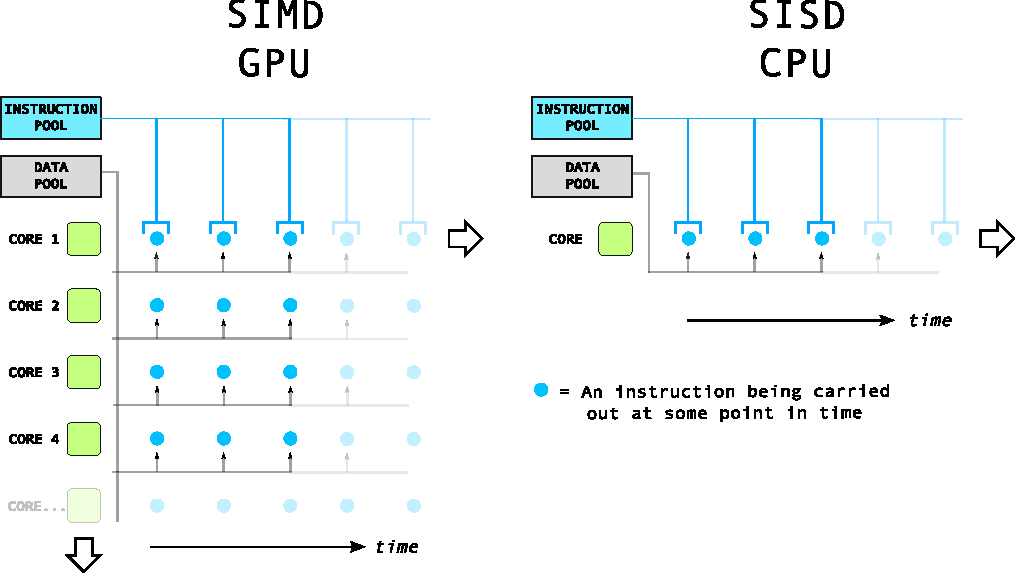
\includegraphics[width=1.0\textwidth]{img/execution_path_newfontv3.pdf}	
	\end{center}
  \caption{CPUs and GPUs differ greatly from one-another. A GPU is a SIMD computing architecture (left), and a CPU is a SISD architecture (right). The CPU has one computing core carrying out the instructions of a program sequentially. A GPU, in contrast, has several computing cores working on the same instruction but with different data for each core.}
	\label{fig:EXE_PATHS}
	%\vspace{-5pt}
\end{figure}

\indent As portrayed in~\cref{fig:EXE_PATHS} there is a fundamental difference in how CPUs and GPUs process their workload. This has its explanation in the fundamental difference between the SISD and SIMD architectures which is also apparent in the number of cores these devices possess\footnote{The cores are all crammed onto a single die/chip. In the case of the CPU, this die is connected directly to the host (motherboard). For a GPU the die is connected to a graphics card, which in turn is connected to the host.}; as of 2010 a typical consumer grade CPU has up to six cores while a GPU has several hundreds\footnote{The NVIDIA GeForce GTX 480 has 480 cores running at 1401 MHz, and the ATI Radeon HD 5870 has 1600 cores at 850MHz. The Intel Core i7-970 CPU has six cores at 3200MHz.}. Furthermore, this translates to a significant difference in theoretical performance in terms of floating point operations per second (FLOPS)\nomenclature{FLOPS}{Floating Point Operations per Second}, which is proportional to the number of cores and the core operating frequency. However, it should be noted that this gage does not give a good measure of real-world performance, but it does give a hint. Refer to~\cref{app:FLOPS} for a more in-depth explanation of FLOPS.


\indent FLOPS can be a performance limiter for computationally intensive algorithms, but in many cases memory bandwidth (MBW)\nomenclature{MBW}{Memory Bandwidth} is the bottleneck~\cite{Ryoo:2008:OPA:1345206.1345220}. MBW is analogous to the speed at which data is transferred back and forth between the computing cores and device memory. An important part of GPU programming therefore revolves around constructing algorithms that minimize memory transfers and redundant use of stored data. \Cref{app:MBW} gives a more thorough explanation of memory bandwidth. \Cref{tab:specs} shows some key attributes for a few mainstream graphics cards and specialized hardware, including theoretical  FLOPS and MBW for single and double precision operations. 

%Memory band width. Refer to appendix~\ref{app:MBW} for ATI's Radeon HD 5870 can for example process 2,72 TFLOPS, NVIDIAs Geforce GTX 480 peaks at 1,34 TFLOPS\\

%the GPU keeps grabbing commands (instructions and data bundled together) from a queue (sent from the CPU) which it executes. If the queue is empty, then the GPU idles.


\begin{table}[htbp]
\caption{Comparison of computational hardware. The interpretation of FLOPS and MBW  is discussed in \cref{app:FLOPS,app:MBW} respectively. Double precision (DP)\nomenclature{DP}{Double Precision} throughput is considerably lower than single precision (SP)\nomenclature{SP}{Single Precision} throughput for these devices. Note that FLOPS are generally not regarded as an accurate measure of actual performance.  \label{tab:specs}}

\begin{center}
\scalebox{0.85}{
% consider including SFU FLOPS
	\begin{tabular}{p{1.6cm}p{1.6cm}p{1.6cm}p{1.3cm}p{1.6cm}p{1.6cm}p{1.6cm}p{1.6cm}}
		\textbf{Model} & \textbf{Year} & \textbf{Release price} [USD] & \textbf{Cores} & \textbf{Frequency} [MHz] & \textbf{FLOPS (SP)} [TFLOPS]& \textbf{FLOPS (DP)} [TFLOPS]& \textbf{Bandwidth} [GB/s]\\
		\toprule[2px]			
		NVIDIA GTX 480 & March 26, 2010 & \$499 & 480 & 1401 & 1.345 & 0.168 & 177.4\\
		\hline
		NVIDIA GTX 470 & March 26, 2010 & \$349 & 448 & 1215 & 1.089 & 0.136 & 133.9\\
		\hline
		ATI/AMD Radeon HD 5870 & September 23, 2009 & $>$\$300 & 1600 & 850 & 2.720 & n/a & 153.6\\%0.544(?)
		\hline
		ATI/AMD Radeon HD 5850 & September 30, 2009 & $>$\$300 & 1440 & 725 & 2.088 & n/a & 128\\%0.418(?)
		\hline
		NVIDIA M2070 & Q2, 2010 & $>$\$4000 & 448 & 1150 & 1.288 & 1.030 & 150.3\\
		%\hline
		%AMD 1095T (CPU) & April 2010 & \$295 & 6 & 3200 & 0.017\footnote{SSEx} & 0.013 & -\\
		%http://www.maxxpi.net/results/show.php?ID=v5y9d8g5p4l3
		%Intel Core i7-970 & July 19, 2010 & \$885 & 4 & 3200 & - & - & -\\
		%\hline
		%Intel Core i7-950 & May 31, 2009 & \$294 & 6 & 3070 & - & - & -\\			
		\bottomrule[2px]	
	\end{tabular}
}	
\end{center}

\end{table}

%This is somewhat alleviated by the core clock frequency which is lower for GPUs.

%In computing, FLOPS (or flops or flop/s) is an acronym meaning FLoating point OPerations per Second. The FLOPS is a measure of a computer's performance, especially in fields of scientific calculations that make heavy use of floating point calculations.
%As of 2010, the fastest PC processors six-core has a theoretical peak performance of 107.55 GFLOPS (Intel Core i7 980 XE) in double precision calculations. GPUs are considerably more powerful. For example, NVIDIA Tesla C2050 GPU computing processors perform around 515 GFLOPS in double precision calculations while AMD FireStream 9270 peaks at 240 GFLOPS. In single precision performance, NVIDIA Tesla C2050 computing processors perform around 1.03 TFLOPS while AMD FireStream 9270 cards peak at 1.2 TFLOPS. Both NVIDIA and AMD's consumer gaming GPUs may reach higher FLOPS. For example, AMD’s HemlockXT 5970 reaches 928 GFLOPS in double precision calculations with two GPUs on board while NVIDIA GTX480 reaches 672 GFLOPS with one GPU on board.


\section{Architecture}
In order to understand the ins and outs of GPU computing it is necessary first to have a basic understanding of the underlying hardware architecture. The architecture depends on manufacturer and model, but from a programming point of view it is  the quantitative rather than the qualitative attributes that differ. Most newer graphics cards from both NVIDIA and ATI can run almost the exact same code due to qualitatively similar architectures. However, a code that is optimized for one architecture might not be optimal for a different one.  \Cref{sec:gpulayout,sec:wg} go through some crucial concepts that follow as a consequence of hardware architecture.

%-But also that there  can only be a very limited amount of talk between the members of such a process. 
\subsection{GPU layout}
\label{sec:gpulayout}
The GPU die is divided in several small subsections as shown in~\cref{fig:hw_layout}. Each of these regions constitute a {\it compute unit}. Each compute unit consists of many\footnote{The NVIDIA GTX 480 and 470 have 32 single precision processing elements per compute unit. The ATI HD 5870 has 80. There are in addition special processing elements for some mathematical functions.} smaller cores, or {\it processing elements}, that carry out most of the arithmetic operations. The processing elements in a compute unit can talk to each other and share data using a small cache\footnote{A memory reservoir used to temporarily store data that will be used a lot is often referred to as a {\it cache}. Caches traditionally trade size for speed.} of {\it local memory}, which is very fast.  The compute units can not communicate with each other. %This constraint is a limiting factor for the type of problems that are currently suitable for GPU programming. 

\begin{figure}[htbp]
	\begin{center}
	\vspace{-10pt}
  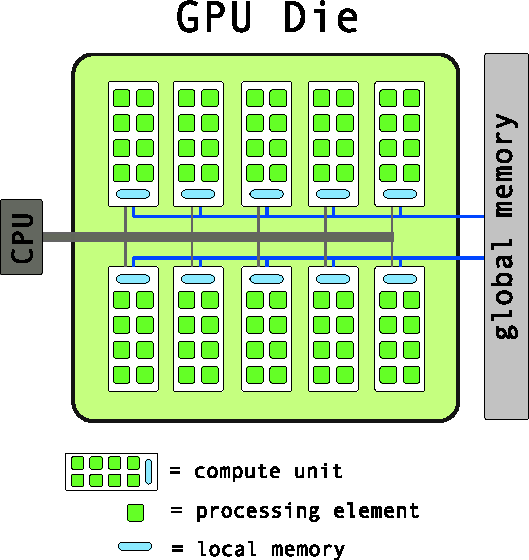
\includegraphics[width=0.5\textwidth]{img/GPU_arch.pdf}
	\end{center}
  \caption{A boiled-down representation of a GPU die showing some of the more essential parts. The CPU sends  instructions to the compute units consisting of i.a. processing elements and local memory. Global memory is accessible both by the host and the compute units. A CPU sends instructions to the compute units.}
	\label{fig:hw_layout}
	\vspace{-5pt}
\end{figure}


\indent A number of caches and control units such as registers, memory controllers, special function units, load/store units, and instruction schedulers occupy the rest of the die space. However, their functions generally fall outside the scope of this discussion. Moving off the chip there is a huge memory reservoir called {\it global memory}. Global memory is both much larger and much slower than local memory. It is used mainly to store input data before a program is invoked and to store results before they are read by the host. 
%They can also be synchronized to avoid erroneous reads and writes from this cache.

\subsection{The work group hierarchy}
\label{sec:wg}
The code that is sent to a GPU is called a {\it kernel} and consists of a sequence of instructions that is forwarded in segments to the compute units. The compute unit then dispatches the instructions to the processing elements.

\indent The kernel running on a processing element is called a {\it work item}, and the programmer can make a group of them map to the same compute unit. These work items form a {\it work group} and can share data through the compute unit's local memory cache as illustrated in~\cref{fig:the_wg}. %The number of work items in a work group should be a multiple of 32 and should not exceed a certain value\footnote{ The maximum number of work items in a work group is typically 1024 for 2010's enthusiast graphics cards.}.\\

%\begin{wrapfigure}{r}{0.4\textwidth}
\begin{figure}[htbp]
	\begin{center}
	\vspace{-10pt}
  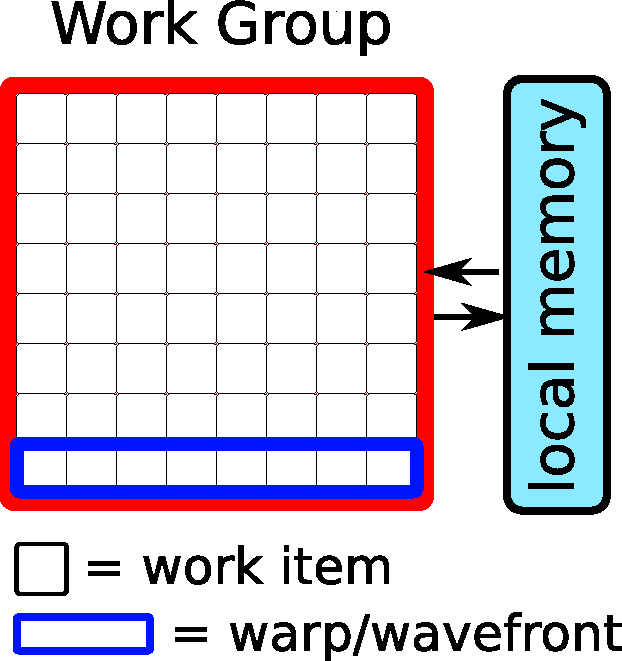
\includegraphics[width=0.30\textwidth]{img/work_group.pdf}
	\end{center}
  \caption{The work group consists of multiple work items assigned to one compute unit that can share data through local memory. Work items are serviced by the processing elements warp by warp.}
	\label{fig:the_wg}
	\vspace{-5pt}
\end{figure}
%\end{wrapfigure}

\indent Work items within a work group are processed in clusters corresponding to the number of processing elements on the compute unit.  NVIDIA has named these clusters {\it warps}, while ATI calls them {\it wavefronts}.  In the remainder of this text these clusters will be referred to as warps. Work items are always serviced together in batches like this. Furthermore, warps can be left to idle while waiting for memory transfers to complete and thus allowing for other warps to be serviced in the meantime. The size of a work group should be a multiple of the size of a warp to keep all processing elements active\footnote{As an example, the NVIDIA GTX 480 has a warp size of 32.  The work groups should therefore be of size 32$n$ where $n = 1,2,3...,48$. The upper limit of $n = 48$ arises due to a hardware limit of 1536 resident work items on a compute unit.}.

% WARPS: No one has fully explained this, but we assume it is because (in the pre-Fermi world) the half-warp is some kind of low level scheduling unit in the hardware. At the software level, we have to treat the warp as the unit of scheduling, but the hardware is free to have slightly finer granularity if that makes sense for the implementation. 

\indent Each work item can be distinguished by unique {\it indices} both within the work group and the grid. For example, the index can be used to access specified addresses in local or global memory.


\indent The programmer decides how much work is done by each work item when writing the kernel, and naturally the work should be distributed so that the number of work groups is greater than the number of compute units to prevent any of them from idling. 
%Section explains how memory latencies can be further reduced by having each compute unit work on several work groups.
It is also possible for a compute unit to work on several work groups at once to hide memory latencies. This  will be examined in~\cref{sec:NDRange}.

\indent Together the work groups make up a grid as shown in~\cref{fig:the_grid}. The dimensions of the work groups and grid have no real significance other than being a convenience when working with multidimensional problems. Still, the total number of work items in a work group,  and of work groups in a grid, has important consequences as described in~\cref{sec:NDRange}.

%\begin{wrapfigure}{r}{0.4\textwidth}
\begin{figure}[htbp]
	\begin{center}
	\vspace{-10pt}
  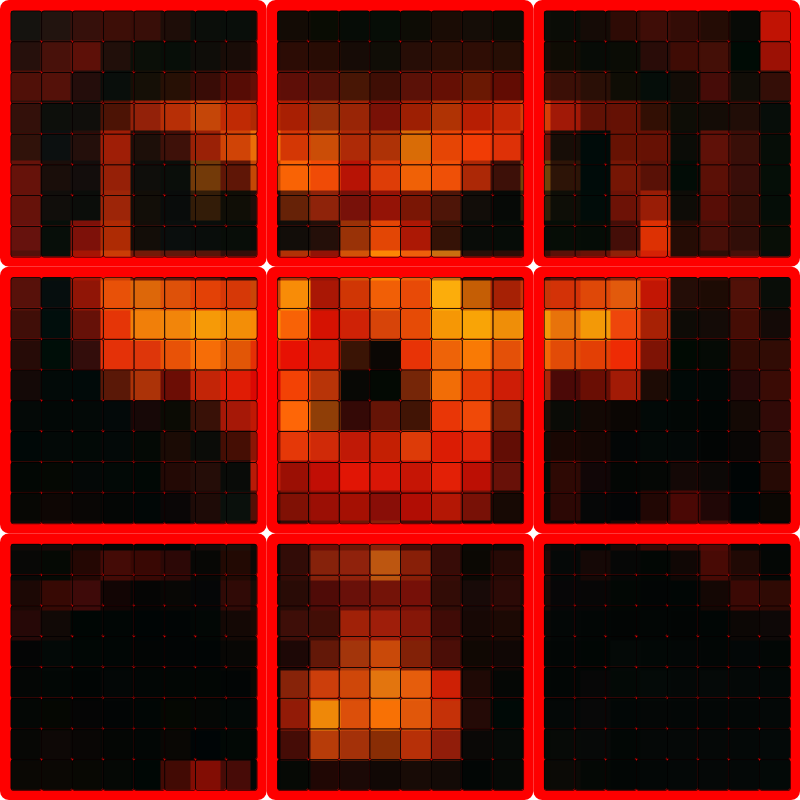
\includegraphics[width=0.45\textwidth]{img/grid_lol.png}
	\end{center}
  \caption{The work groups that are needed to solve a problem form a grid. The dimensions of the grid can easily be mapped to a multidimensional problem for the sake of convenience. One example is to let the grid span over an image and have each work item represent a pixel as shown here.}
	\label{fig:the_grid}
	\vspace{-5pt}
\end{figure}
%\end{wrapfigure}



\section{OpenCL}
OpenCL\footnote{Abbreviation for Open Computing Language.} is a framework for writing programs that execute across platforms consisting of CPUs, GPUs, and other processors. OpenCL includes a language for writing kernels and application programming interfaces\footnote{An application programming interface is an interface implemented by a software program that enables it to interact with other software.} (APIs)\nomenclature{API}{Application Programming Interface} that are used to define and then control the platforms~\cite{OpenCL.spec}.

\indent OpenCL is developed and maintained by the member-funded Khronos Group that works to create open standards for graphics, media and parallel computation. Many well known hardware manufacturers are member of the group, and NVIDIA, AMD/ATI, and Intel are among them. The main argument for using OpenCL instead of other APIs is the open standard that makes it much more portable than for example the CUDA API from NVIDIA or the Stream API from AMD/ATI, which are limited t.

%Debugging
%\indent Part of OpenCL is implementation defined, meaning that some behavior is allowed to vary between conforming implementations of OpenCL: For example the error of a mathematical function.

%Vendor dependent things called ***
\subsection{PyOpenCL}
PyOpenCL~\cite{PyOpenCLweb} accesses the OpenCL parallel computation API from Python~\cite{10.1109/MCSE.2007.58}, a high level open source programming language. Python is especially convenient as an upper level code layer due to its clean syntax and broad functionality.

\section{Performance Optimization\label{sec:performance}}
This section highlights why optimization is essential to achieve appreciable performance in general purpose GPU computing and gives a few examples of how it can be realized. The following paragraphs first describes high priority optimization factors and then proceeds to briefly discuss some  that  are normally less important. The content is largely based on guides from NVIDIA~\cite{opencl.best.practices, opencl.programming} and ATI~\cite{ATIguide}.


%Which strategies will yield the best performance gain for a particular portion of an
%application depends on the performance limiters for that portion; optimizing
%instruction usage of a kernel that is mostly limited by memory accesses will not yield
%any significant performance gain, for example. Optimization efforts should
%therefore be constantly directed by measuring and monitoring the performance
%limiters,

\subsection{Structuring an Algorithm}
Evidently, the algorithm has to be written for parallel execution: There are several processing elements working at the same time on a work group, and the kernel should be written in such a way  that the work is equally distributed among the work items. For example, if a work group needs to load some data and has 256 work items, then all those should fetch $1/256$ of that data each, and, depending on the problem, either do the necessary operations on that data or store it in local memory to be shared with the other work items. This is an example of parallelization. \Cref{code:parallel} shows how a simple code changes from a sequential to a parallel implementation. 

\begin{figure}[htbp]
	\vspace{-20pt}
	\begin{center}
	\begin{lstlisting}[language=C, style=my_C]
	for(int i = 0; i < N; i++){
		out_data[i] = in_data[i];
	}
	\end{lstlisting}
	\vspace{-20pt}
	\begin{lstlisting}[language=C, style=my_C]
	int i = get_global_id(1); //get unique work item index
	out_data[i] = in_data[i];
	\end{lstlisting}
\caption{Top: A sequential implementation of an algorithm that copies an array of length $N$. Bottom: The corresponding parallel implementation. Each of the $N$ work items copies one element. Note that a for-loop is unnecessary since the programmer has already specified the number of work items that should carry out the task. \label{code:parallel}}
\end{center}

\end{figure}


\indent Generally, during the optimization process it is important to be aware of significant performance limiters. For example, optimizing instruction usage of a kernel that is mostly limited by memory accesses will not result in any significant performance gain. NVIDIA and ATI offer free proprietary software that can be used to monitor these performance limiters. Also, for larger kernels, it is recommended to  optimize heavier parts of the code first, since this is where the largest gain in performance can be obtained. 

\indent Memory transfer involving  global memory is a costly operation in terms of clock cycles compared to transfers within local memory and most arithmetic operations. The algorithm should therefore be constructed in a way that minimizes redundant memory access, or even better, reduces memory access altogether. Global memory latency can be hidden if sufficiently many arithmetic instructions can be issued while waiting for the transfer to complete. However, this is only possible for certain types of problems. The ratio of clock cycles spent for the arithmetic operations to the number of clock cycles spent for load/store operations will be referred to as arithmetic density in this text.
%-Distributing the work within a WG
%-Minimize transfer between host and device. Do it on the GPU, not the CPU!
%-Focus on optimizing the heavy parts

\subsection{Global Memory}
\label{sec:global_mem}
Input and output data has to be stored in global memory before and after a kernel is invoked, respectively. Assuming the algorithm has already been designed to minimize global memory transfer, substantial performance losses can still occur if the data is not accessed in a way that agrees on a hardware level.

\indent Global memory is divided in several {\it memory banks} that are accessed from each compute unit, and if two memory access requests go to the same memory bank, hardware serializes the access. This is commonly referred to as a {\it bank conflict}. When data is written to global memory, consecutive elements are stored in consecutive memory banks. It is therefore preferred to access this data in the same order it was stored to minimize serialization. This is called {\it coalesced access}. As an example, if only every second element in an array of data was read, only half of the memory banks would contribute to transfer the data that was actually requested. A common term for this event is {\it strided access}, and in the former example the stride was two. \Cref{code:strided_access} shows a kernel with strided access, and~\cref{fig:strided_access} displays the resulting effect on global memory bandwidth.

\begin{figure}[htbp]
	\vspace{-20pt}
	\begin{center}
	\begin{lstlisting}[language=C, style=my_C]
	__kernel void strided_access(
	__global const float* in_data,
	__global float* out_data,
	int stride)
	{	
		int i = get_global_id(1);
		out_data[i] = in_data[i*stride];
	}
	\end{lstlisting}
\caption{A kernel that copies elements stored in global memory. Strided access can be achieved by changing {\it stride} to a desired value as shown in~\cref{fig:strided_access}.\label{code:strided_access}}
\end{center}

\end{figure}

\begin{figure}[htbp]
	\vspace{-20pt}
	\begin{center}
		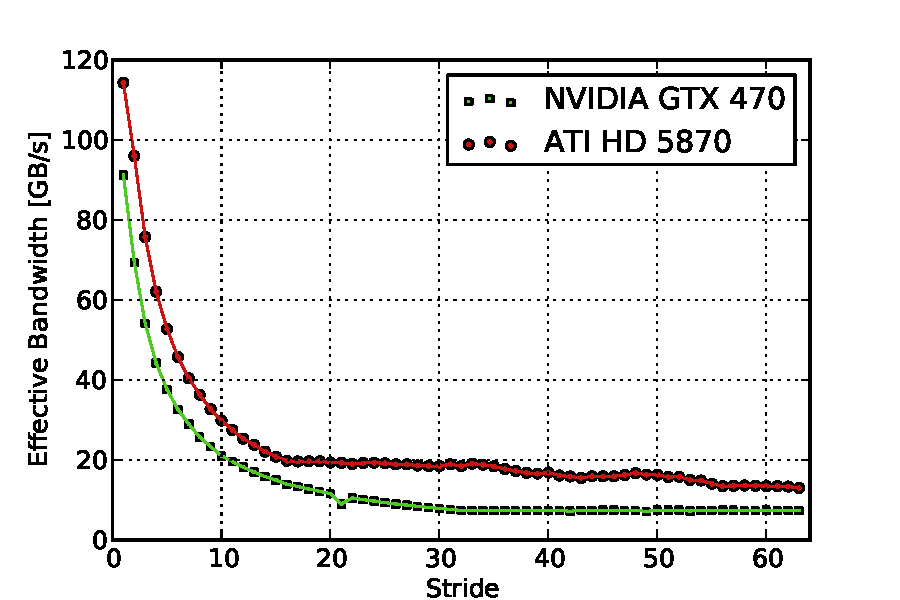
\includegraphics[width=0.70\textwidth]{img/strided_access.pdf}		
	\end{center}
	\vspace{-10pt}
	\caption{Strided access severely impaired the memory bandwidth of the graphics cards included in this test.}
	\label{fig:strided_access}
\end{figure}




\indent When data is stored in global memory, successive words\footnote{{\it Word} is the term used for the natural unit of data for a given architecture. For example, on a 32-bit system, each word has a size of 32-bits, and memory transfers are therefore done in in segments of 32 bits. A single precision value is 32 bits and therefore has the size of exactly one word on a 32-bit system. A double precision value is 64 bits and therefore has the size of exactly two words on a 32-bit system, but only one word on a 64-bit system. Note that a compute unit loads or stores several words at once.} are stored in successive memory banks, but there is only a limited number of memory banks.  Work items in a warp ideally read from unique banks without any bank conflicts. However, data is always read in segments of successive words that span over several memory banks, the first part of an array being the first segment etc.. A warp that accesses words stored in two or more segments might have to read both segments in their entirety, spending twice as much time. For example, a warp that reads elements 1 to 32 in an array of length 64 stored in two segments (as opposed to elements 0 to 31) might\footnote{Some recent graphics cards tend to mitigate or circumvent some of the issues with misaligned access by caching memory transactions~\cite{opencl.programming}.} have to read them both. This is called {\it misaligned access}. \Cref{fig:strided_misaligned} gives a graphical overview of both strided and misaligned access patterns.


%\begin{wrapfigure}{r}{0.4\textwidth}
\begin{figure}[htbp]
	\begin{center}
	%\vspace{-5pt}
  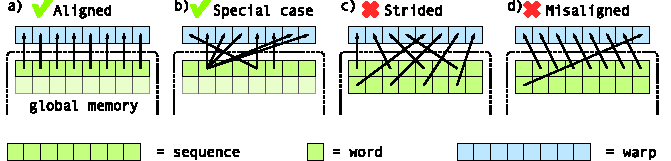
\includegraphics[width=1\textwidth]{img/strided_misaligned.pdf}
	\end{center}
  \caption{{\bf a)} Aligned and coalesced access of global memory. {\bf b)} There is no penalty in the case where the same memory address is accessed by multiple elements of the same warp. {\bf c)} Strided access does not take full advantage of the hardware parallelism due to bank conflicts. The stride in this example is two.  {\bf d)} Misaligned access forces the processing elements to read the first sequence in addition to a great part of the last one.}
	\label{fig:strided_misaligned}
	%\vspace{-5pt}
\end{figure}
%\end{wrapfigure}



\indent On a final note, some of the kernel's input data may be of a predictable nature, and it should be considered to reconstruct it within the kernel instead of reading it from global memory.
%On a final note, if some of the kernel's input data resides in global memory, but is of a predictable nature, it should be considered to reconstruct it within the kernel instead of reading it from global memory.
%some input data may be of a predictable nature, and it should be considered to reconstruct it within the kernel instead of reading it from global memory. %\todo{Does this report have too many "if"s?}


%-Minimize use of (400-600 CS vs 8 CS) and thus increase Arithmetc density - 
%-Coalesced access to
%-Recomputing data
\subsection{Local Memory}
Recall from~\cref{sec:wg} that each compute unit administers a small cache of on-chip local memory.  Local memory is substantially faster than global memory\footnote{For a 2009 GPU from NVIDIA, the throughput of memory operations was 8 operations per clock cycle, but there was in addition a latency of 400 to 600 clock cycles when accessing global memory. The latency for accessing local memory was approximately a factor of 100 lower.~\cite{opencl.best.practices}.}, and it is a good idea to use local memory for caching data that will be used more than once within a work group or to store some intermediate results. Doing so helps reduce redundant transfers involving global memory and can greatly improve performance.  The lifespan of data stored in local memory is the same as the lifespan of the work group that used it.
% \todo{Possibly include a typical example and a plot showing the difference in speed (MBW) using naive and enhanced implementations. Maybe a transpose or matrix multiplication.}

\indent Data sent to local memory is stored in multiple memory banks and is therefore vulnerable to strided access.  Therefore, if multiple addresses of a memory request map to the same memory bank, the accesses are serialized. However, there is no bank conflict between work items accessing the same element in a bank.

\indent When one instruction of a kernel invocation writes a word to local memory, and the successive instruction for some other work item involves reading the same data, there is no guarantee that the given word is actually stored before it is read. However, the work items can be forced to synchronize by raising a {\it memory fence} in-between the two events. \Cref{code:barrier} displays code and possible output for two such scenarios. Memory fences cost additional clock cycles and force processing elements to idle while waiting for each other. They should therefore be used sparsely. 

\begin{figure}[htbp]
	\vspace{-20pt}
	\begin{center}
	
{\bf{\ttfamily\selectfont in\_data = [   0.    1.    2.    3.   ...   63.   64.   65.   66.   ...   125.  126.  127.]}}

	\begin{lstlisting}[language=C, style=my_C]
	__kernel void flip(
	__global const float* in_data,
	__global float* out_data,
	__local float* cache)
	{
		int i = get_local_id(1);
		cache[i] = in_data[i];
		out_data[i] = cache[127-i];
	}
	\end{lstlisting}

%{\bf out\_data = [ 127.  126.  125.  124.  . . .  64.    {\color{bloody}0.    0.    0.}  . . .  2.    1.    0.]}
{\bf{\ttfamily\selectfont out\_data = [ 127.  126.  125.  124.  ...  64.    {\color{bloody}0.    0.    0.}  ...  2.    1.    0.]}}

	\begin{lstlisting}[language=C, style=my_C]
	__kernel void barrier_flip(
	__global const float* in_data,
	__global float* out_data,
	__local float* cache)
	{
		int i = get_local_id(1);
		cache[i] = in_data[i];
		// Raise memory fence 
		barrier(CLK_LOCAL_MEM_FENCE);		
		out_data[i] = cache[127-i];
	}
	\end{lstlisting}

%{\bf out\_data =  [ 127.  126.  125.  124.  . . .  64.   63.   62.   61.  . . .  2.    1.    0.]}
{\bf{\ttfamily\selectfont out\_data =  [ 127.  126.  125.  124.  ...  64.   63.   62.   61.  ...  2.    1.    0.]}}

\caption{Two kernels attempt to flip an array of 128 elements, but the former is not guaranteed to give the correct result due to the lack of a synchronization point. A synchronization point is introduced by adding the 
command {\tt barrier(CLK\_LOCAL\_MEM\_FENCE)}.\label{code:barrier}}
\end{center}

\end{figure}


\subsection{Execution Paths}
Any flow control instruction, such as {\bf if}, {\bf while}, {\bf for}, {\bf switch}, or {\bf do}, can potentially force work items within a warp to take different execution paths. If this happens, the different
executions paths will be serialized and executed sequentially, increasing the total number of instructions
executed for the warp and leaving a number of processing elements idle. When all the different execution paths have completed, the work items converge back to the same execution path. Substantial performance improvements can be realized by taking care that the code seldom requires work items in a warp to diverge. In other words, a work group can execute disjoint code paths at no extra cost as long as its warps do not.


%Care should be taken not to create divergent paths unless strictly necessary or the performance hit is negligible\todo{Are threads locked to the same warp over the entire life-span of a work group? Wouldn't that contradict some of their acclaimed predictability?}.


%Write conflicts can be avoided using atomic functions. Atomic functions get serialized within a warp. 


%Branch divergence
%occurs only within a warp; different warps execute independently regardless of
%whether they are executing common or disjoint code paths.


%. The way a block
%is partitioned into warps is always the same; each warp contains threads of
%consecutive, increasing thread IDs with the first warp containing thread 0.
%Section 2.1 describes how thread IDs relate to thread indices in the block.


%-divergent warps and flow control
%Example 2: If t is the time it takes to execute a single iteration of a loop; and
%within a wavefront all work-items execute the loop one time, except for a single
%work-item that executes the loop 100 times, the time it takes to execute that
%entire wavefront is 100t.

%Example 1: If two branches, A and B, take the same amount of time t to execute
%over a wavefront, the total time of execution, if any work-item diverges, is 2t.
%Loops execute in a similar fashion, where the wavefront occupies a compute unit
%as long as there is at least one work-item in the wavefront still being processed.

\subsection{NDRange and Occupancy\label{sec:NDRange}}

Registers are fast on-chip memory units that store variables declared by the kernel. Each compute unit has a fixed number of registers to distribute among its resident work groups, and as long as there are enough free registers a compute unit will continue to launch concurrent work groups. Local memory is used on a per-work-group basis, meaning there also has to be sufficient local memory in order for several work groups to spawn.
When the processing elements on a compute unit invoke a memory transfer for a warp they can put the warp aside and execute instructions for other warps while out-waiting the memory latency. This allows for completely hiding latency from registers and local memory (and to some extent global memory). The more active warps the more latency can be hidden away.

\indent There are hardware limits to the maximum number of active work groups, warps, and work items on a compute unit. The ratio of resident warps to the maximum number of resident warps given by the hardware limit is called {\it occupancy}, and it is used as a performance gage since GPU devices typically need a certain occupancy to completely hide register latency. Choosing execution parameters such as the work group size, register usage, and local memory usage is a matter of striking a balance between latency hiding and resource utilization. For example, while having a work group use only part of the available local memory can help hide latency, it often means more redundant memory transfers.

\indent NDRange is a term used in OpenCL to describe the dimensions of the work groups and grid for a specific kernel invocation. While these dimensions can be practical in order to more conveniently project a multidimensional problem, cf.~\cref{fig:the_grid}, they have no impact on performance. The size, however, does: The number of work groups in a grid should be greater than, and preferably a multiple of, the number of compute units so that none of them can idle.  In addition, there should be multiple active work groups per compute unit so that work groups that are not waiting for a memory fence can keep the hardware busy. To scale to future devices, the number of work groups per kernel launch should be in the hundreds, as kernels with thousands of work groups will scale across multiple future GPU generations~\cite{opencl.best.practices}.  For kernels where each work group take approximately the same amount of time to execute, the number of work groups should be a multiple of the number of compute units to avoid the last batch of work groups to occupy only a fraction of the compute units. 

%Maybe say something about preferred work group sizes
\subsection{Loop Unrolling\label{sec:unroll}}

As this report will show later, loop unrolling can sometimes help to greatly improve performance. Unrolling a loop means  increasing the quantity of instructions per iteration by reducing the number of iterations. Doing so not only reduces conditional checks of the loop overhead; it also helps the compiler to coalesce fetch and store instructions if these are placed in adjacent code lines as shown in~\cref{code:unroll_example}. However, doing so also taxes the registers since registers are not freed up until the variables they hold are no longer needed. \Cref{fig:unroll_performance} shows the performance differences between the two kernels in~\cref{code:unroll_example}. The two kernels do the exact same job, but one of them a loop has been unrolled by a factor of four. The optimal unrolling factor for a kernel generally is considered to be a parameter for experimentation. 



\begin{figure}[htbp]
	\vspace{-20pt}
	\begin{center}
		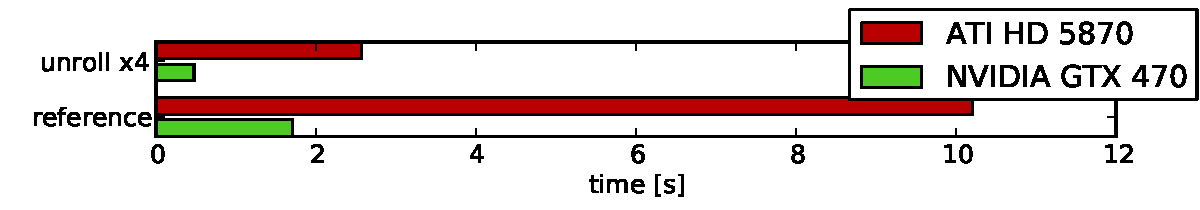
\includegraphics[width=\textwidth]{img/unroll_performance.pdf}		
	\end{center}
	\vspace{-10pt}
	\caption{Performance for the kernels shown in~\cref{code:unroll_example} for an array of $N = 256,000$ randomly generated numbers and $loopCount = N$. Unrolling by a factor of four improved performance substantially on the graphics cards included in this test.\label{fig:unroll_performance}}
	
\end{figure}



\begin{figure}[htbp]
	\vspace{-20pt}
	\begin{center}

	\begin{lstlisting}[language=C, style=my_C]
	__kernel void normal_loop(
	__global const float* in_data,
	__global float* out_data,
	uint loopCount)
	{
		uint i = get_global_id(1);
		for(uint j = 0; j < loopCount; j++){			
			out_data[i] += in_data[j];					
		}		
	}
	\end{lstlisting}
\vspace{-25px}
	\begin{lstlisting}[language=C, style=my_C]	
	__kernel void unrolled_loop(
	__global const float* in_data,
	__global float* out_data,
	uint loopCount)
	{
		uint i = get_global_id(1);
		for(uint j = 0; j < loopCount; j+=4){
			float X0 = in_data[j];
			float X1 = in_data[j+1];
			float X2 = in_data[j+2];
			float X3 = in_data[j+3];

			out_data[i] += X0;	
			out_data[i] += X1;			
			out_data[i] += X2;			
			out_data[i] += X3;							
		}		
	}
	\end{lstlisting}


\caption{The first kernel shows a regular for-loop. The next shows the same loop unrolled by a factor of four (the kernels add some elements of an array to each element of that same array and have no use other than being instructive). Performance comparisons are shown in~\cref{fig:unroll_performance}.\label{code:unroll_example}}
\end{center}

\end{figure}




%ATI's HD 5870 is vastly outperformed due to an intelligent cache design by NVIDIA.(Needs confiramtion, but the L2 cache might have played a key part here)

% fetch/store coalescing at the cost of registers
% http://forums.nvidia.com/index.php?showtopic=50508
%-Helping the compiler? 
%-pragma unroll
%Maximum number of instructions per kernel


\newpage
\subsection{Native Math Library And Compilation Flags}
\label{sec:native}
Some mathematical functions, like {\tt sin}, {\tt cos} and {\tt sqrt} to name a few, can be replaced by native device instructions by appending the  {\tt native\_} prefix. Native functions typically have better performance compared to their standard versions, but at the cost of precision. The accuracy and behavior of such functions are implementation defined. \Cref{fig:native_functions} gives an impression of how the {\tt sin} function varies from the {\tt native\_sin} function in terms of performance, for example. \Cref{fig:native_functions_STD}  shows the standard deviation of the same functions using C++ generated  double precision CPU calculations as a reference.

\indent On a final note, OpenCL offers a number of optional compilation flags that trade precision for speed. Discretion is advised.

\begin{figure}[htbp]
	\begin{center}
		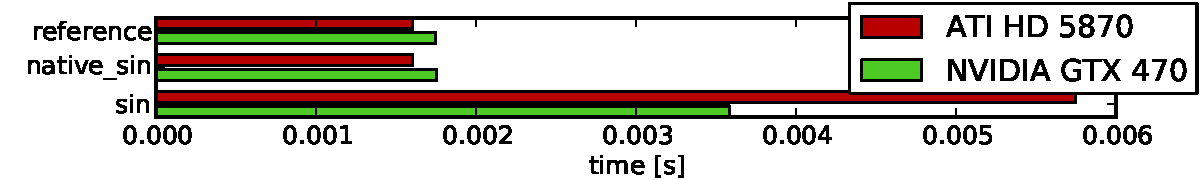
\includegraphics[width=\textwidth]{img/native_functions.pdf}		
	\end{center}
	\vspace{-10pt}
	\caption{Performance for an implementation defined native function on two graphics cards. The reference kernel copies an array of $25,600,000$ randomly generated single precision numbers. The two other kernels calculate {\tt sin} and {\tt native\_sin}, respectively, for each element of the same array before copying it. The kernel that calculates {\tt native\_sin} is limited by global memory bandwidth.}
	\label{fig:native_functions}
\end{figure}

\begin{figure}[htbp]
	\vspace{-5pt}
	\begin{center}
		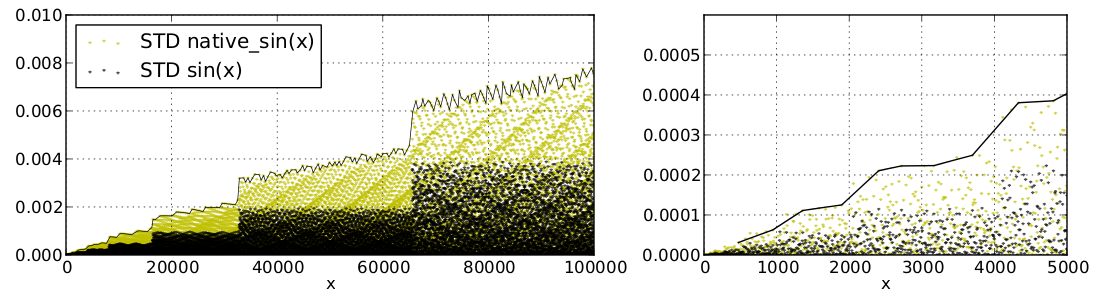
\includegraphics[width=\textwidth]{img/NVIDIA_native_functions_MSE.png}		

		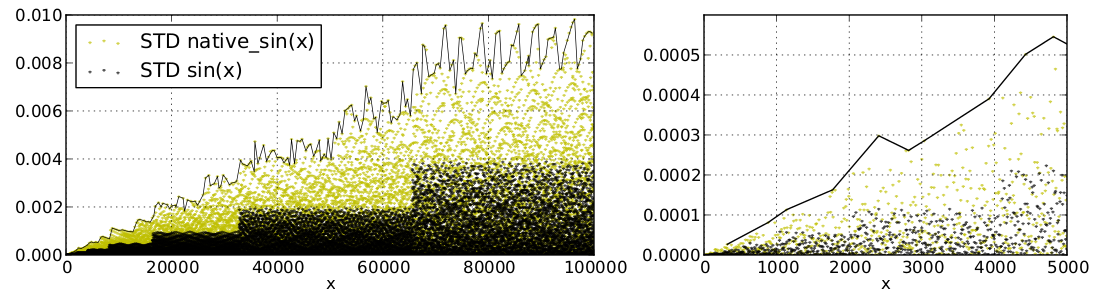
\includegraphics[width=\textwidth]{img/ATI_native_functions_MSE.png}		
	\end{center}
	\vspace{-10pt}
	\caption{The standard deviation for {\tt sin(x)} and {\tt native\_sin(x)} in single precision as a function of $x$ using C++ generated  double precision CPU calculations as a reference. The continuous black lines trace the maximum values of the standard deviation for {\tt native\_sin(x)}. Top: NVIDIA GTX 470.  Bottom: ATI HD 5870.}
	\label{fig:native_functions_STD}
\end{figure}



%\subsection{Miscellaneous}

%\begin{itemize}

%\item 

%\item Avoid integer division and modulo operators and substitute them with bitwise operations whenever possible as they are particularly costly. If $n$ is a power of $2$, $(i/n)$ is equivalent to $(i>>\log2(n))$ and $(i \% n)$ is equivalent to $(i \& (n-1))$.

%\item ...
%
%\end{itemize}
%\subsubsection{Avoiding division and modulo operators}
%Shift operations
%\subsubsection{Inverse square root}



\chapter{X-ray Theory}
This chapter gives an introduction to the physics of the Debye equation without going into excessive detail. The chapter begins with an explanation of X-ray scattering and continues to explain how this phenomenon can be used to obtain structural information.  The chapter proceeds with the derivation of the Debye formula, which can be used to simulate wide angle and small angle X-ray scattering from orientationally averaged systems, such as powders of identical and randomly oriented particles or objects in solution. The last section describes a slightly rewritten  and computationally less demanding version of this equation.

\section{Scattering}
When X-rays interact with matter, any given photon has a certain chance to be scattered by the electron cloud that surrounds the atoms. Many materials exhibit periodic structure at the atomic scale and consequently a periodic electron distribution. Constructive and destructive interference occurs when the periodic structures of such materials scatter electromagnetic radiation in or out of phase, respectively. For example, if two initially coherent photons of the same energy are scattered in the same direction, they will experience a relative phase shift $\phi$, and if $\phi$ = $2n\pi$ their amplitudes will interfere constructively ($n \in 0,  \pm1, \pm2...$). $\phi$ = $(2n+1)\pi$, on the other hand, corresponds to destructive interference. The phase shifts occur because photons are deflected by different atoms when they scatter, introducing spatial variations between their paths. This phenomenon, which falls under the collective term {\it diffraction}, is fundamental in X-ray scattering. 

\indent X-ray diffraction basically involves a source, a monochromator, a collimator, a sample, and a detector. A monochromatic beam of nearly parallel X-rays is incident on a sample and the scattered radiation is measured by a detector at different angles and sample orientations. The resulting plot of intensity vs. angle holds a lot of information about the sample. Moreover, it has peaks for angles of constructive interference, but tends to diminish for angles of low or destructive interference. However, in order to interpret the results it is much more convenient to treat scattering in reciprocal space, or ${\mathbf Q}$-space (as opposed to real-space).
%while the sample and detector are slowly rotated

\indent Using ${\mathbf Q}$-space is a convenient way of representing information, and one which is ideal for studying periodic structures. ${\mathbf Q}$-space is the same as Fourier space and has dimensions of inverse length. Both electromagnetic radiation and periodic electron distributions can  be described by Fourier theory as superpositions of sines and cosines~\cite{kreyszig}, both of which are described by their respective wave vectors. X-rays are described by a wave vector
% that can be described by one or more wave vectors.
\begin{equation}
{\mathbf k}_{Xray} = \frac{2\pi}{\lambda}\widehat{ {\mathbf k}}_{Xray}
\label{eq:k_ray}
\end{equation} 

\noindent where $\lambda$ is the X-ray wavelength and $\widehat{ {\mathbf k}}_{Xray}$ is a unit vector in the direction of the ray. Periodic electron distributions, that is, crystal lattices, are described by reciprocal lattice vectors
\begin{equation}
{\mathbf G} = \frac{2\pi}{\|{\mathbf d}\|}\widehat{{\mathbf d}} ,
\label{eq:k_lattice}
\end{equation} 

\noindent where ${\mathbf d}$ is an inter-atomic spacing vector in real space.  \Cref{fig:scattering} shows a periodic lattice in ${\mathbf Q}$-space with an incoming X-ray ${\mathbf k}_{i}$. Note that the reciprocal lattice is actually the ${\mathbf Q}$-space representation of the electron distribution of the real space lattice. The scattered X-ray, denoted by ${\mathbf k_{f}}$, can take any direction, but the kinetic energy remains constant in the scattering process. The Laue condition~\cite{xrayphys} states that a necessary condition for constructive interference is

\begin{equation}
{\mathbf Q} \equiv {\mathbf k}_{f} - {\mathbf k}_{i} = {\mathbf G} ,
\label{eq:laue}
\end{equation} 

\noindent which is true only for certain scattering angles. 


\begin{figure}[htbp]
	%\vspace{-5pt}
	\begin{center}
		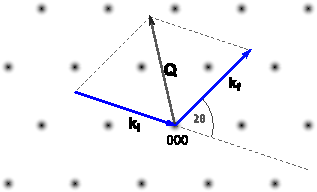
\includegraphics[width=0.5\textwidth]{img/scattering.pdf}			
	\end{center}
	\vspace{-10pt}
	\caption{An incoming X-ray  ${\mathbf k}_{i}$ is scattered by an atomic lattice plane, which is represented in ${\mathbf Q}$-space by a reciprocal lattice. The scattered X-ray is denoted by ${\mathbf k}_{f}$. If ${\mathbf Q}$ coincides with a reciprocal lattice vector, there will be constructive interference and a bright, observable reflection in the direction of the corresponding ${\mathbf k}_{f}$.  \label{fig:scattering}}
\end{figure}



The sphere spanned by ${\mathbf Q}$ in~\cref{fig:scattering_ewald} is titled the Ewald sphere and has the property that ${\mathbf Q} = {\mathbf G}$ in the places where it intersects with the reciprocal lattice. In other words, X-rays that exit with ${\mathbf k}_{f}$ such that ${\mathbf Q} = {\mathbf G}$ yield bright reflections. 

\begin{figure}[htbp]
	%\vspace{-5pt}
	\begin{center}
		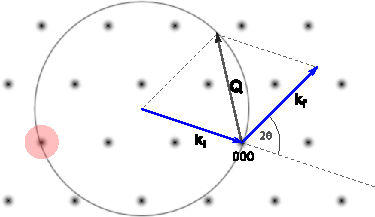
\includegraphics[width=0.5\textwidth]{img/scattering_ewald.pdf}		
	\end{center}
	\vspace{-10pt}
	\caption{The Ewald sphere shows which ${\mathbf k}_{f}$ can be expected to produce constructive interference by fulfilling the Laue condition ${\mathbf Q} = {\mathbf G}$. In the illustrated case the Ewald sphere intersects with the reciprocal lattice in one single place (marked by a red spot), and the corresponding ${\mathbf k}_{f}$ may therefore yield a bright reflection.\label{fig:scattering_ewald}}
\end{figure}



\indent In basic powder diffraction experiments with a stationary source, the sample and detector can be rotated about collinear axes at angular speeds $\omega$ and $2\omega$, respectively. In such setups  the angle $2\theta$ between ${\mathbf k}_{i}$ and ${\mathbf k}_{f}$  changes, thus scanning the intensity $I({\mathbf Q})$ for a specific range of ${\mathbf Q}$. The sample is rotated  such that ${\mathbf Q}$ keeps its direction with respect to the reciprocal lattice, so it is only the magnitude of ${\mathbf Q}$ that changes during the scan. By simple geometry the conversion from the angle between ${\mathbf k}_{i}$ and ${\mathbf k}_{f}$, namely $2\theta$, and the corresponding magnitude of ${\mathbf Q}$, is given by

\begin{equation}
Q = 2\|{\mathbf k}\|\sin{\theta}  = \frac{4\pi}{\lambda}\sin{\theta} 
\label{eq:thetatoq}
\end{equation} 

\indent If the sample is a powder consisting of randomly oriented particles, the reciprocal lattice will take a corresponding number of  different orientations around its origin, smearing out discrete lattice points to spherical shells. The resulting intersections with the Ewald sphere are rings that form diffraction patterns like the one shown in~\cref{fig:scattering_powder}. The same figure shows a cross section of a similar pattern,  displaying the intensity as a function of $Q$. The patterns can be used   to find inter-atomic spacings through~\cref{eq:k_ray,eq:k_lattice}.

\begin{figure}[htbp]
	\vspace{-10pt}
	\begin{center}
		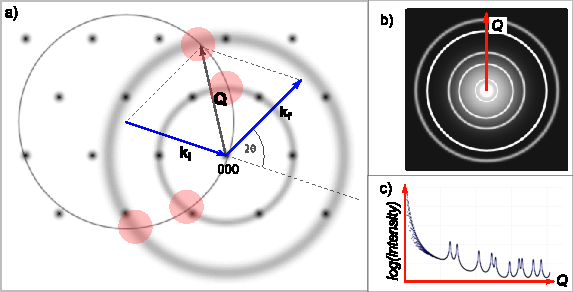
\includegraphics[width=\textwidth]{img/scattering_powder.pdf}	
	\end{center}
	\vspace{-10pt}
	\caption{In powder diffraction the particles can take any orientation resulting in a reciprocal space filled with spherical shells rather than points ({\bf a}). As a result the intersections between the reciprocal lattice and the Ewald sphere form rings that allow cone-shaped shells of X-rays to escape the powder and give bright reflections. The resulting image is a ring-shaped pattern ({\bf b}). A radial average of a similar pattern ({\bf c}), called a diffractogram, displays the intensity as a function of $Q$.\label{fig:scattering_powder}}
\end{figure}


\indent The relative phase of a scattered X-ray is generally given by


\begin{equation}
e^{i({\mathbf k}_{f} - {\mathbf k}_{i})\cdot{\mathbf r}_{j}} = e^{i{\mathbf Q}\cdot{\mathbf r}_{j}} ,
\label{eq:phase}
\end{equation} 


\noindent where ${\mathbf r}_{j}$ is the position of the $j$th atom. For a group of atoms\footnote{This is not restricted to a periodic lattice.} the scattering amplitude is proportional to the structure factor given by

\begin{equation}
F({\mathbf Q}) = \sum_{i} f_{j}(Q)e^{i{\mathbf Q}\cdot{\mathbf r}_{j}} ,
\label{eq:F}
\end{equation} 

\noindent where $f_{j}(Q)$ is the presumably spherically symmetric atomic form factor of the $j$th atom, given by the integral

\begin{equation}
f({\mathbf Q}) = \int \rho({\mathbf r})e^{i{\mathbf Q}\cdot{\mathbf r}}\mathrm{d}^{3}{\mathbf r} ,
\label{eq:atomic_form_factor}
\end{equation} 

\noindent where $\rho({\mathbf r})$ denotes the electron density. The atomic form factor characterizes the specific atom's electron distribution and thus its ability to scatter X-rays. Furthermore, the scattering intensity $I({\mathbf Q})$ from a group of $N$ atoms, when disregarding correction factors, is equal to the structure factor squared,

\begin{equation}
I({\mathbf Q}) = |F({\mathbf Q})|^{2} = \sum_{i=1}^{N}\sum_{j=1}^{N} f_{i}({\mathbf Q})f_{j}({\mathbf Q})e^{i{\mathbf Q}\cdot{\mathbf r}_{ij}} ,
\label{eq:FF}
\end{equation} 

\noindent where ${\mathbf r}_{ij} \equiv {\mathbf r}_{i}-{\mathbf r}_{j}$.

\section{Debye Formula}
\label{sec:debye}
\Cref{eq:FF} describes diffraction from one particle made up from $N$ atoms. The Debye formula~\cite{xrayphys}, in contrast, describes diffraction from an aggregate of such particles taking all possible rotations in space. Noting that the orientational average of $e^{i{\mathbf Q}\cdot{\mathbf r}}$ is


\begin{equation}
{\Big\langle e^{i{\mathbf Q}\cdot{\mathbf r}} \Big\rangle  } = \frac{\sin{Qr}}{Qr} ,
\label{eq:debye0}
\end{equation} 

\noindent the Debye formula is readily obtained:

\begin{equation}
I(Q) = \sum_{i=1}^{N}\sum_{j=1}^{N} f_{i}(Q)f_{j}(Q)\frac{\sin{Qr_{ij}}}{Qr_{ij}}
\label{eq:debye1}
\end{equation} 

\noindent Note that all vectors have changed to scalar values. The output of the Debye formula is a diffractogram as shown in~\cref{fig:scattering_powder}, or in other words, a plot of $I(Q)$. 
\Cref{eq:debye0} is based on the following assumptions:
\begin{itemize}
\item Incoming X-rays scatter only once (Kinematical approximation~\cite{xrayphys}).
\item X-rays scatter elastically.
\item The particles are perfectly randomly oriented.
\end{itemize}

\noindent The last assumption is sometimes problematic in paractice, but the first two are generally considered to be excellent~\cite{xrayphys}.

\indent Exploiting the symmetry properties $r_{ij} = r_{ji}$ and\footnote{Note that $ \lim_{x\to0} \sin(x)/x = 1$.} $r_{ii} = r_{jj} = 0$, the Debye formula simplifies to 

\begin{equation}
\boxed{
I(Q) = \sum_{k=1}^{N}f_{k}^{2}(Q) + 2\sum_{i=1}^{N-1}\sum_{j=i+1}^{N} f_{i}(Q)f_{j}(Q)\frac{\sin{Qr_{ij}}}{Qr_{ij}}} 
\label{eq:debye}
\end{equation} 


\noindent which is still a computationally heavy function for large $N$ with the number of calculations scaling as $N(N-1)/2 \approx N^{2}/2 \propto N^{2}$.

\indent In order for the synthetic results obtained from~\cref{eq:debye} to be comparable to real world measurements, it is necessary to introduce some correction factors~\cite{ springerlink:10.1134/S1063783407010246, xrayphys}. However, such comparisons are not in the scope of this report. %These appear as correction factors and are known as the Lorentz, Polarization, and Geometrical %corrections . By multiplying~\cref{eq:debye} with an angular factor

%\begin{equation}
%LPG(\theta) = \frac{1 + \cos{2\theta}^2}{4\sin{2\theta}\sin{\theta}},\hspace{14px}  \mbox{where} \hspace{6px} %\theta = \arcsin{\frac{Q\lambda}{4\pi}}
%\label{eq:lpg}
%\end{equation} 

%said corrections are taken into account.


\section{Specific Formulation}
\label{sec:spec_debye}
The Debye~\cref{eq:debye} allows for all $N$ atoms of a particle to take different atomic form factors. However, from a computational point of view this is not a desirable situation because each of the $N(N-1)/2$ contributions to $I(Q)$ then depend on two variables, $f_{i}(Q)$ and $f_{j}(Q)$, that have to be loaded from memory for all $N(N-1)/2$ computations. 

\indent It is both convenient and logical to limit the problem to a small number of atom types since in any case there cannot be more types of atoms in a particle than there are elements, or strictly, ions.  In order to benefit from this limitation the atoms can be arranged by their respective form factors as shown in~\cref{fig:problem_space}. The atomic form factors can then be factored out of~\cref{eq:debye0,eq:debye} for the various combinations of atoms.



\indent It is apparent from~\cref{fig:problem_space} that the combinations of atoms generate both triangular and rectangular regions of computations.  Denoting the respective atom types of a particle by $m$ and $n$, the contribution $I_{mn}(Q)$ to $I(Q)$ from the rectangular regions where $m \neq n$ is given by

\begin{equation}
%I_{mn}(Q) = f_{m}(Q)f_{n}(Q)\sum_{i=N_{m,i}}^{N_{m,f}}\sum_{j=N_{n,i}}^{N_{n,f}} \frac{\sin{Qr_{ij}}}{Qr_{ij}} ,
I_{mn}(Q) = f_{m}(Q)f_{n}(Q)V(Q),
\label{eq:rectangle}
\end{equation} 

\noindent where

\begin{equation}
%I_{mn}(Q) = f_{m}(Q)f_{n}(Q)\sum_{i=N_{m,i}}^{N_{m,f}}\sum_{j=N_{n,i}}^{N_{n,f}} \frac{\sin{Qr_{ij}}}{Qr_{ij}} ,
V(Q) = \sum_{i,j} \frac{\sin{Qr_{ij}}}{Qr_{ij}} ,
\label{eq:rectangle_inner}
\end{equation} 

\noindent and $i$ and $j$ run over all atoms of type $m$ and $n$, respectively. For the triangular regions where $m = n$,~\cref{eq:rectangle} reduces to

\begin{equation}
%I_{mn}(Q) = f_{m}^{2}(Q)\sum^{N_{m,f}}_{N_{m,i}}1 + 2f_{m}^{2}(Q)\sum_{i=N_{m,i}}^{N_{m,f}-1}\sum_{j=i}^{N_{m,f}}
%\frac{\sin{Qr_{ij}}}{Qr_{ij}} ,
I_{mm}(Q) = N_{m}f_{m}^{2}(Q) + 2f_{m}^{2}(Q)W(Q),
\label{eq:square}
\end{equation} 

\noindent where

\begin{equation}
%I_{mn}(Q) = f_{m}^{2}(Q)\sum^{N_{m,f}}_{N_{m,i}}1 + 2f_{m}^{2}(Q)\sum_{i=N_{m,i}}^{N_{m,f}-1}\sum_{j=i}^{N_{m,f}}
%\frac{\sin{Qr_{ij}}}{Qr_{ij}} ,
W(Q) = \sum_{i=1}^{N_{m}-1}\sum_{j=i+1}^{N_{m}} \frac{\sin{Qr_{ij}}}{Qr_{ij}} 
\label{eq:square_inner}
\end{equation} 

\noindent and $N_{m}$ denotes the number of atoms of type $m$. 

\begin{figure}[htbp]
	%\vspace{-10pt}
	\begin{center}
		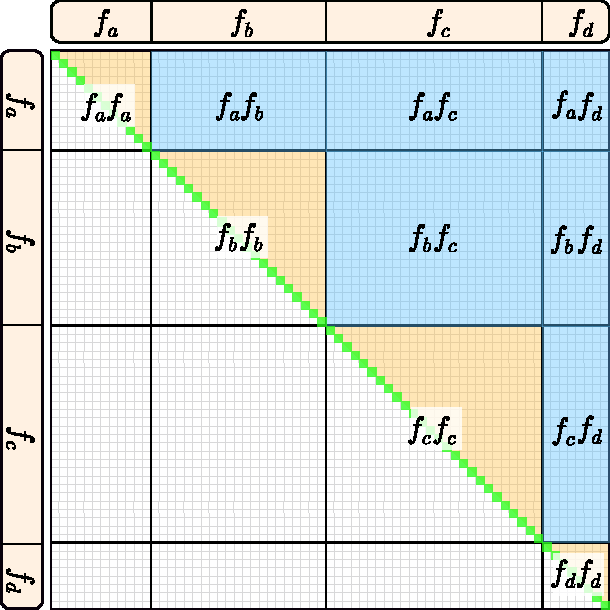
\includegraphics[width=0.7\textwidth]{img/calculation_structure.pdf}	
	\end{center}
	%\vspace{-10pt}
	\caption{The problem space of the Debye equation for a lattice consisting of four different atom types (represented here by four atomic form factors). The total intensity $I(Q)$ is given by~\cref{eq:i_sum_symm}. For the triangle-shaped instances where $f_{m}(Q) = f_{n}(Q)$ the intensity contributions can be obtained from~\cref{eq:square}. The contributions from the rectangular tiles are given by~\cref{eq:rectangle}. Due to symmetry, no computations are necessary for the white area.\label{fig:problem_space}}
\end{figure}

\indent$I(Q)$ for a powder of the particles can then be expressed as
%These groups will be referred to as {\it tiles} for the remainder of the report. 
\begin{equation}
I(Q) = \sum_{m=1}^{M}\sum_{n=1}^{M} I_{mn}(Q) 
\label{eq:i_sum}
\end{equation} 

\noindent where $M$ is the total number of atom types. Using the symmetry property $I_{mn}(Q) = I_{nm}(Q)$,~\cref{eq:i_sum} reduces to

\begin{equation}
I(Q) = \sum_{m=1}^{M}I_{mm}(Q) +   2\sum_{m=1}^{M-1}\sum_{n=m+1}^{M} I_{mn}(Q)  
\label{eq:i_sum_symm}
\end{equation} 

\noindent \Cref{eq:i_sum_symm} is the basis for an algorithm that can calculate $I(Q)$ for any powder of particles that satisfies the assumptions given in~\cref{sec:debye}. The particles can be of any composition and there is no requirement that their lattice is periodic, allowing the inclusion of strain, lattice defects, unusual shapes and other nanoscale features. 



\chapter{X-ray Scattering Simulation}
This chapter describes how a Debye algorithm was implemented in OpenCL to achieve appreciable performance on GPUs. The first section gives some perspective on the problem and outlines the implementation in some detail.  There is also a short description of the Python framework used to  generate an atomic lattice and administer communication between the host and the GPU. 

\section{Initial Considerations\label{sec:initial_considerations}}
The Debye equation gets increasingly laborious for large numbers of atoms $N$ with the number of calculations scaling as $N(N-1)/2$. Furthermore, it might be desirable to have hundreds of data points (values of $I(Q)$), if not thousands. Denoting the number of data points by $N_{Q}$ brings the total number of calculations to $N_{Q}N(N-1)/2$. For example, a spherical \chem{CoO} particle with a diameter of $10$ nm consists of close to  $\num{5.4e4}$ atoms, amounting to more than $\num{1.45e9}$ calculations of the type
%a high-resulution diffractogram might have
\begin{equation}
\operatorname{sinc}{Qr_{ij}} = \frac{\sin{Qr_{ij}}}{Qr_{ij}}
\label{eq:inner_calc}
\end{equation} 

\noindent for each data point. A \chem{CoO} particle with a diameter of $20$ nm has more than $\num{4.3e5}$  atoms ($8\times$ the previous particle) and needs a total of $\num{9.3e10}$ calculations ($8^{2}\times$ as many as for the previous particle).  Furthermore, calculating \cref{eq:inner_calc} involves several arithmetic and load/store operations. For two atoms $i$ and $j$ with coordinates $(x_{i},y_{i},z_{i})$ and $(x_{j},y_{j},z_{j})$, the distance between them is

\begin{equation}
r_{ij} = \sqrt{(x_{i}-x_{j})^{2} + (y_{i}-y_{j})^{2} + (z_{i}-z_{j})^{2}},
\label{eq:norm}
\end{equation} 


\noindent meaning that each calculation involving two new atoms  will load at least six separate values from memory in addition to storing a result.  Since load/store operations generally take much longer than arithmetic operations, it is reasonable that memory latency  could have some impact on performance. Also note that the $Q$-values can easily be reconstructed by the kernel as discussed in~\cref{sec:global_mem}. In order to reduce redundant access of memory it is therefore tempting to calculate \cref{eq:inner_calc} for all $Q$ once $r_{ij}$ has been computed and the positions of two atoms have been loaded. Furthermore, if each work item was told to compute \cref{eq:inner_calc} for {\it one} pair of atoms, the work items could use local memory to share atom position data and to add up temporary results for different values of $Q$ before storing the results in global memory. Continuing, the work items could replace one of their two atoms with a new one and calculate a new $r_{ij}$ before repeating the former steps until all combinations $ij$ had been cycled through. Even though this would help maximize the arithmetic density for the given problem, there is one issue: Several work items and work groups could potentially read from and write to the same locations in memory {\it at the same time}, which would cause erroneous results due to read/write conflicts. It can be argued that this problem is avoidable by careful loop handling and/or use of parallel reduction. However, it is still possible to aim for high arithmetic density, and thus performance, by using a tuned-down version of the previous example, adjusted to prevent read/write conflicts.

\indent \Cref{eq:inner_calc} contains a sine, a square root and a division, all of which can be substituted by native functions as described in~\cref{sec:native}. However, the accompanying precision losses must be considered. Loop unrolling should be implemented (\cref{sec:unroll}), and the grade of unrolling should be a variable parameter to allow for experimentation. It should also be possible to indirectly adjust the usage of local memory and registers to ease the search of a balance between occupancy and usage of  these resources. The implementation should also show good scalability to future GPUs. One way to achieve this is to split the workload between at least several hundred work groups as explained in~\cref{sec:NDRange}.   

%\noindent the minimum number of arithmetic operations required to compute a single data point is:

%\begin{itemize}
%\item One sine
%\item One division
%\item One square root
%\item Four multiplications
%\item Five subtractions and additions
%\end{itemize}

%In addition, at least six load operations are required to load the atom positions, and one store operation for the result. Moreover, in order to get the number of arithmetic operations this low it is necessary to store some temporary variables in the registers.

\section{Dealing With Single Precision} 
One important attribute of most consumer grade graphics cards is that they are optimized for single precision data (i.e.\ 32-bit words). Note that graphics cards have their origin in the gaming industry where they were only needed to render graphics without the special need for high precision. In numerics, however, precision is often crucial.  

\indent Precision can be defined as the smallest floating point number $\epsilon$ that, when added to the floating point number 1.0, produces a number different from 1.0. 32-bit single precision floating point numbers have $\epsilon \approx \num{1.19e-7}$, and double precision 64-bit floating point numbers have $\epsilon \approx \num{2.22e-16}$~\cite{numrec}.
 While it is possible to do calculations in double precision on recent graphics cards, the theoretical FLOPS value is usually much lower than for single precision, cf.~\cref{tab:specs}. The implementation of the algorithm presented in this report is therefore written for single precision computations, and rather tries to reduce the likelihood of erroneous results that arise from adding values of very different magnitude\footnote{Recall that the Debye equation involves a double sum, and therefore a significant number of additions.}. Summarizing the last two sections, the algorithm should in particular focus on the following qualities:  

%Precision is analogous to the number of significant digits. For example, if the single precision value $a = 0.0001$ is added to a value $b = 10000$ of the same accuracy, the result will be equal to $b = 10000$, and not $a+b = 10000.0001$. This happens because $b$ does not have enough significant digits to treat $a$ as anything else than noise. In double precision (two 32-bit words or one 64-bit word), the precision much better, and $a+b$ would indeed give the correct result.
\begin{itemize}
\item Performance 
\item Precision
\item Scalability to future GPUs.
\end{itemize} 

\subsection{Parallel Reduction\label{sec:parallel_reduction}}
Parallel reduction is a way of calculating the sum of the  elements of an array. It attempts to decrease the chance of adding values of substantially different magnitudes by adding adjacent values in several steps. The principle works best for arrays that do not show pronounced trends, such as increasing values along the array. \Cref{fig:par_red} illustrates the working principle of parallel reduction. Furthermore, parallel reduction is very well suited for parallel implementations. 

\begin{figure}[htbp]
	%\vspace{-5pt}
	\begin{center}
		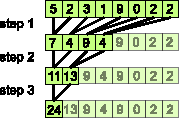
\includegraphics[width=0.5\textwidth]{img/par_red.pdf}		
	\end{center}
	%\vspace{-10pt}
	\caption{In parallel reduction adjacent values of an array are added together in several steps. The array of size eight above requires three steps to produce the result. The final step adds the values $13$ and $11$, whereas a more naive implementation might add up the elements sequentially and finally add $22$ and $2$, for which the difference is greater, thus leaving the addition more vulnerable to precision errors. The size of the array has to be a power of two. Note that the stride is one (\cref{sec:global_mem}). \label{fig:par_red}}
\end{figure}
%N square, memory load, q-loop




\section{Algorithm\label{sec:algo}}
%-Description of working principles
%-Input parameters
%-Native functions, float 3
%\todo{maybe skip sentence from here}

Two different kernels have been written in accordance with~\cref{eq:i_sum_symm}. One of them, the {\it triangle algorithm}, computes $W(Q)$ in~\cref{eq:square}. The second, called the {\it rectangle algorithm}, computes $V(Q)$ in~\cref{eq:rectangle}. The names originate from the two different shapes of the regions where $m = n$ or $m \neq n$ as shown in~\cref{fig:problem_space}. This section gives a description of the kernels.

%apply some of the optimization techniques from~\cref{sec:performance}. to help improve the performance by use. 
%The kernels have been written such that 

\indent The two kernels use the exact same principles except that the triangle algorithm exploits  symmetry properties, effectively halving the time it takes to execute. Each work group is responsible for calculating $V(Q)$ or $W(Q)$ for $N_{Q,wg}$ values of $Q$, cf.~\cref{fig:kernel_grid}. $N_{Q,wg}$ is one of the variable  parameters of the algorithms, and by increasing it the number of memory transfers is reduced by a factor close to $1/N_{Q,wg}$, thereby increasing the arithmetic density.



\begin{figure}[htbp]
	\centering
	\begin{subfigure}{0.7\textwidth}
	  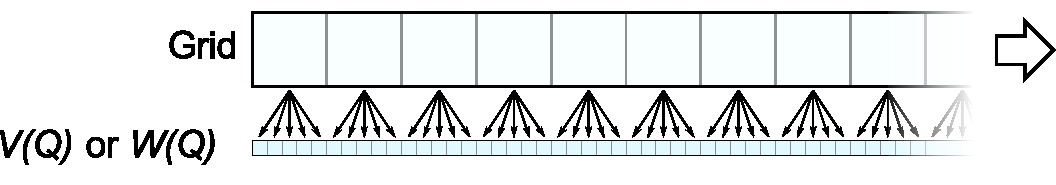
\includegraphics[width=\textwidth]{img/kernel_grid.pdf}
	  \caption{The grid: Each work group computes $V(Q)$ or $W(Q)$ for $N_{Q,wg}$ successive values of $Q$.}
	  \label{fig:kernel_grid}	
	\end{subfigure}
	\vspace{5mm}
	\begin{subfigure}{0.5\textwidth}
	  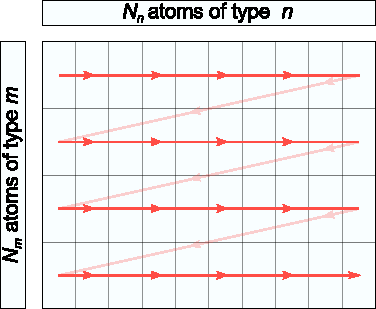
\includegraphics[width=\textwidth]{img/kernel_wg_rect.pdf}
	  \caption{The work groups of the {\it rectangle algorithm} cycle through all available tiles before sending any results to global memory.}
	  \label{fig:kernel_wg_rect}	
	\end{subfigure}
	\hspace{5mm}
	\begin{subfigure}{0.42\textwidth}
	  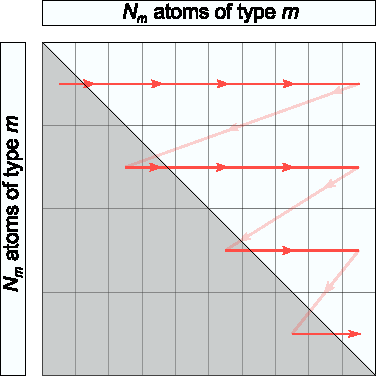
\includegraphics[width=\textwidth]{img/kernel_wg_tri.pdf}
	  \caption{The work groups of the {\it triangle algorithm} avoid any tiles that can be omitted due to symmetry.}
	  \label{fig:kernel_wg_tri}	
	\end{subfigure}
	\vspace{5mm}
	\begin{subfigure}{0.47\textwidth}
	  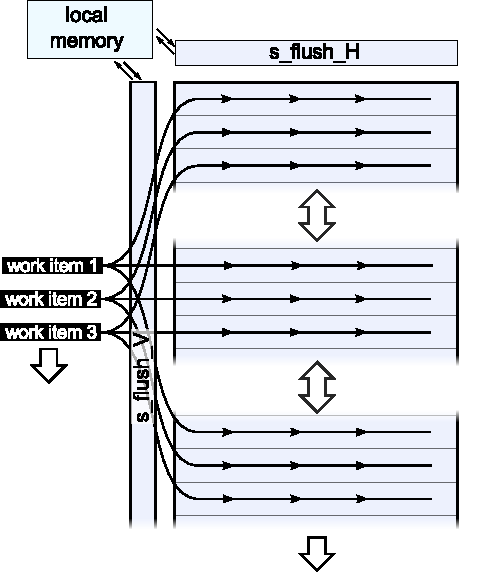
\includegraphics[width=\textwidth]{img/kernel_tile.pdf}
	  \caption{The tile:  All work items in a work group read atom positions from the same pool in local memory.}
	  \label{fig:kernel_tile}	
	\end{subfigure}
	\hspace{5mm}
	\begin{subfigure}{0.47\textwidth}
	  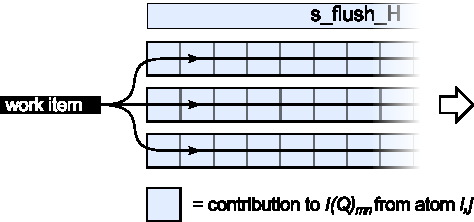
\includegraphics[width=\textwidth]{img/kernel_wi.pdf}
	  \caption{Each of the $N_{wi}$ work items has the ability to calculate $\operatorname{sinc}{Qr_{ij}}$ for several $r_{ij}$ after loading an atom position from  {\tt s\_flush\_H}.}
	  \label{fig:kernel_wi}	
	\end{subfigure}
	\caption{ Two slightly different algorithms, namely the {\it rectangle} and the {\it triangle algorithm}, calculate~\cref{eq:square_inner} or~\cref{eq:rectangle_inner} respectively.}
\end{figure}

\indent When a work group calculates $V(Q)$ or $W(Q)$ it divides the problem into multiple sub-regions, called {\it tiles}, as shown in~\cref{fig:kernel_wg_rect,fig:kernel_wg_tri}. Each tile loads a number of atom positions from global memory ($stride = 1$) and stores them in the local memory cache in the form of two arrays\footnote{The {\tt V} and {\tt H} in {\tt s\_flush\_V} and {\tt s\_flush\_H} stand for {\it vertical} and {\it horizontal}. {\tt s\_flush} comes from {\it store} and {\it flush}.} {\tt s\_flush\_V} and  {\tt s\_flush\_H}, cf.~\cite{gpugems}. The number of atom positions stored in these two arrays defines the size of the tile. Their respective sizes are multiples of the number of work items per work group since they are accessed by all work items at once.

\indent Throughout the lifetime of a tile the $N_{wi}$ work items in the work group need to access the same atomic data several times, but since it is cached and freely accessible, it no longer has to be loaded from global memory for each request. The way this works is illustrated in~\cref{fig:kernel_tile}: After transferring the data from global to local memory, each work item loads data corresponding to a few atom positions from {\tt s\_flush\_V} such that the entire array is in use. Next, the work items all load a single atomic position from {\tt s\_flush\_H} and calculate \cref{eq:inner_calc} for $N_{Q,wg}$ different values of $Q$. This procedure is followed until each item in {\tt s\_flush\_H} has been processed (cf.~\cref{fig:kernel_wi}), at which time the data in {\tt s\_flush\_H} is replaced and the next tile is initialized.  Note that $N_{wi}$ is one of the variable parameters of the algorithms, as are the number of atomic positions in {\tt s\_flush\_V} and  {\tt s\_flush\_H}.  %these atom positions without the extra cost reading them all data from global memory, since 

\indent Increasing the size of {\tt s\_flush\_V} by a factor $K$ makes each work item calculate \cref{eq:inner_calc} for $N_{Q,wg}$ values of $Q$ for $K$ atom positions {\it for each atomic position} loaded from {\tt s\_flush\_H}. This mechanism has been implemented as a fully unrolled for-loop that is unrolled by a factor $KN_{Q,wg}$.  Note that $K$ equals the length of {\tt s\_flush\_V} divided by the number of work items per work group.

\indent When several work items calculate $\operatorname{sinc}{Qr_{ij}}$ for the same value of $Q$ (but different $r_{ij}$), the results are stored in an array in local memory of length $N_{wi}$ to prevent the situation where several work items attempt to add their results to the same memory address, cf.~\cref{sec:initial_considerations}. Moreover, there has to be $N_{Q,wg}$ such arrays, meaning  $N_{Q,wg}$ is capped since there is a finite and relatively small amount of local memory. The last action a the tile takes is to sum elements of each array using parallel reduction and add the results to a vector in global memory, cf.~\cref{fig:kernel_grid}. Afterwards, the data stored in {\tt s\_flush\_H} is replaced with another segment of atomic data, defining a new tile.

\indent Note that the procedure of calculating $V(Q)$ or $W(Q)$ involves the sequential addition of $K$ instances of \cref{eq:inner_calc}. These (small) sums are added to the vectors in local memory for each atomic position in {\tt s\_flush\_H}, at which time  the elements of each array are summed using parallel reduction. Each tile follows the same procedure and always finishes by adding $N_{Q,wg}$ contributions to $V(Q)$ or $W(Q)$ in global memory. The combined effects of parallel and segmented addition help mitigate the errors resulting from working in single precision.

\indent The triangle algorithm avoids computations for  tiles that can be omitted due to symmetry as shown in~\cref{fig:kernel_wg_tri}. For those tiles that are split between the excludable and non-excludable regions, only the relevant computations are carried out.

\indent On a final note, any {\tt sin} function or floating point division has been replaced by {\tt native\_sin} and {\tt native\_divide}, respectively (cf.~\cref{sec:native}).

% The algortihms have also been set to use the {\tt -cl-mad-enable} compilation flag that allows $a\cdot b + c$ to be replaced by a {\tt mad}.

  


%-q loop fail vs q-loop with atomics
%-naive example
%-full example


\section{Limitations}
%Registers
%Local memory
%What about large N?
%LIMIT on Nq, s_flush_H and s_flush_V.
The algorithms discussed in the prevision section have no limit on the number of atoms for which they can compute $V(Q)$ and $W(Q)$. The hardware, however, does. \Cref{fig:N_glb_mem} shows the relation between use of global memory and the number of atoms. In the  event that a calculation requires more atom positions than  global memory allows, the problem can simply be split into more manageable tasks, i.e.\ more instances of~\cref{eq:square_inner,eq:rectangle_inner}.
\begin{figure}[htbp]
	%\vspace{-10pt}
	\begin{center}
		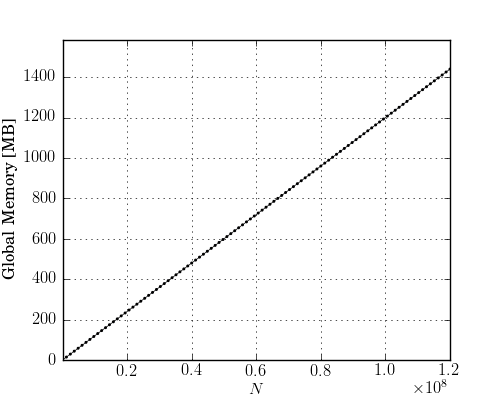
\includegraphics[width=0.5\textwidth]{img/N_glb_mem.png}	
	\end{center}
	%\vspace{-10pt}
	\caption{The algorithms work for relatively large numbers of atoms due to low usage of global memory. The NVIDIA GTX 470 has $1280$ MB of global memory, and the ATI HD 5870 has 1024 MB.\label{fig:N_glb_mem}}
\end{figure}

\indent Of greater consequence is the limited availability of local memory and registers even on recent graphics cards. The impact these limits have on performance is discussed in~\cref{sec:results_perf}.


\section{Framework\label{sec:framework}}
A Python framework is used to produce results from the algorithms and administer any related tasks. \Cref{fig:framework} portrays the various dependencies of the executable script that constitutes the framework.

\begin{figure}[htbp]
	%\vspace{-10pt}
	\centering
		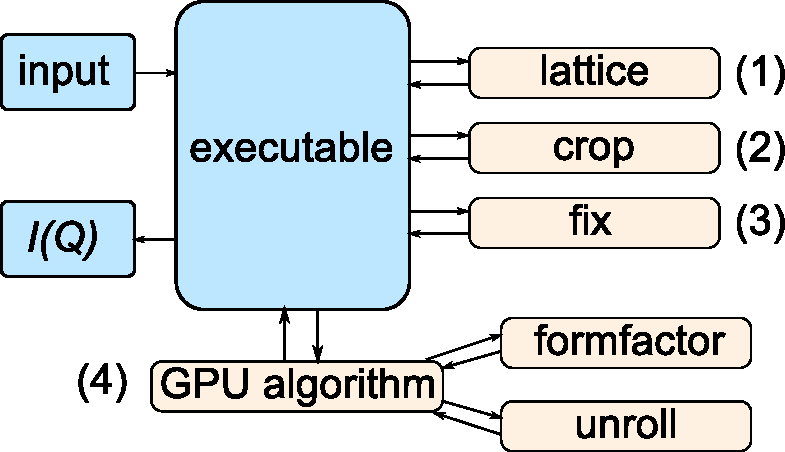
\includegraphics[width=0.7\textwidth]{img/framework.pdf}	
% 	\end{center}
	%\vspace{-10pt}
	\caption{The various dependencies of the executable script that administers the subtasks. Based on the input variables, a Python script generates a lattice (1) and crops it to form a particle (2). Afterwards a few additional atoms are added to help the arrays match the specified NDRange parameters (3). Then the GPU calculates $I(Q)$ (4) with the help of a script that automatically unrolls the algorithm's most critical for-loop and returns a kernel to the GPU. The atomic form factors are loaded from a simple external script, written by Jostein B. Fløystad, and based on parameterizations by Waasmaier and Kirfel~\cite{Waasmaier:sh0059}. \label{fig:framework}}
\end{figure}

\indent The program starts out with the assembly of a particle. This is done by generating a lattice shaped like a rectangular prism of a particular length, width and height, cf.~\cref{fig:uncropped_lattice}. Different atom types are stored in different arrays to keep them separate, which is necessary in order to use~\cref{eq:square,eq:rectangle}. Next, the lattice is cropped so as to form any desired particle shape, for example a sphere as shown in~\cref{fig:cropped_lattice}. The final step before the GPU algorithm is put to work involves padding each array with a few atomic positions such that the array lengths are multiples of {\tt s\_flush\_V} and {\tt s\_flush\_H}, respectively, and thereby fit the NDRange, cf.~\cref{sec:NDRange,sec:algo}. The additional atoms are given positions that are so far away from the original particle and each-other that they will never give any noticeable contributions to the results, cf.~\cref{fig:cropped_fixed_lattice}. Note that \cref{eq:inner_calc} declines quickly for large inter-atomic distances, as shown in~\cref{fig:sinc}. It appears that it is seldom required to add more than a few hundred atoms per array, regardless of the particle size.   

\begin{figure}[htbp]
	\centering
	\begin{subfigure}{0.45\textwidth}
	  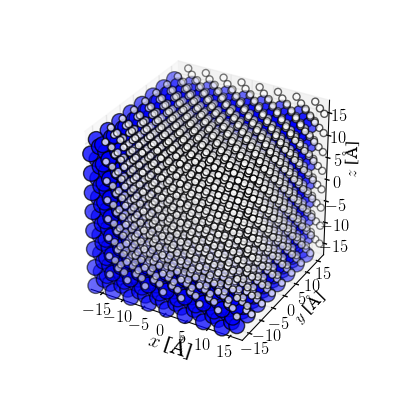
\includegraphics[width=\textwidth]{img/lattice_uncropped.png}
	  \caption{A \chem{CoO} lattice with the shape of a rectangular prism.}
	  \label{fig:uncropped_lattice}	
	\end{subfigure}
	\hspace{5mm}
	\begin{subfigure}{0.45\textwidth}
	  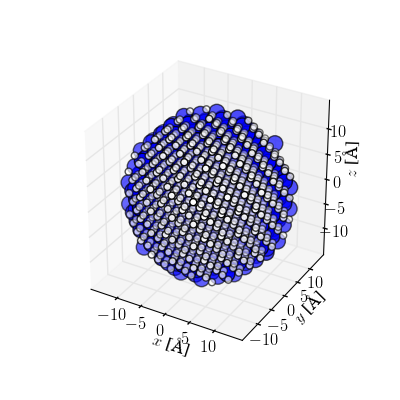
\includegraphics[width=\textwidth]{img/lattice_cropped.png}
	  \caption{A spherical \chem{CoO} particle cut out from the lattice in~\subref{fig:uncropped_lattice}.}
	  \label{fig:cropped_lattice}	
	\end{subfigure}
	\begin{subfigure}{0.45\textwidth}
	  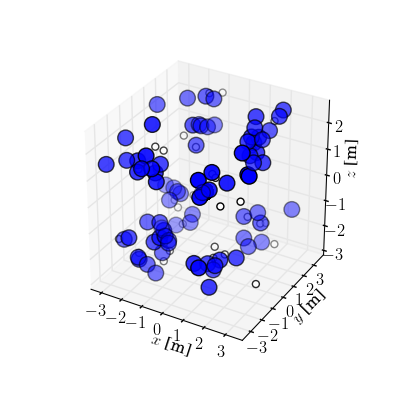
\includegraphics[width=\textwidth]{img/lattice_cropped_fixed.png}
	  \caption{A few additional atoms have been added to locations far away from the particle, which is located in the origin. Note the scale.}
	  \label{fig:cropped_fixed_lattice}	
	\end{subfigure}
	\hspace{5mm}
	\begin{subfigure}{0.4\textwidth}
	  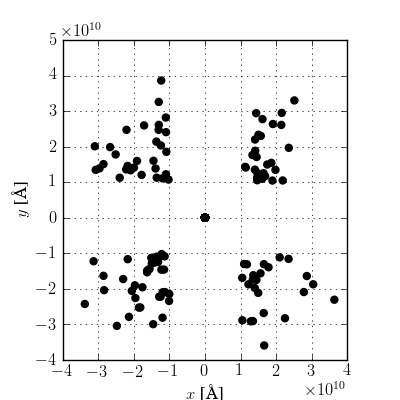
\includegraphics[width=\textwidth]{img/lattice_cropped_fixed_2d.png}
	  \caption{Cross section view of the plot to the left. Note that none of the additional atoms are anywhere
near the particle in the center, and that the inter-atomic distances are relatively large.}
	  \label{fig:cropped_fixed_lattice_d2}	
	\end{subfigure}
	\caption{ The program constructs the desired particle in two steps \subref{fig:uncropped_lattice} and \subref{fig:cropped_lattice}.  The third step adds a few atoms to make the array lengths multiples of {\tt s\_flush\_V} and {\tt s\_flush\_H}, respectively, to fit the NDRange: \subref{fig:cropped_fixed_lattice}, \subref{fig:cropped_fixed_lattice_d2}.}
\end{figure}
 
% \begin{figure}[htpb]
% \centering
% \subfloat[]{\label{fig:uncropped_lattice}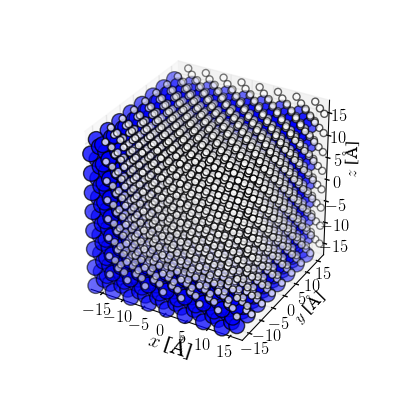
\includegraphics[width=0.45\textwidth]{img/lattice_uncropped.png}}\hspace{20px}
% \subfloat[]{\label{fig:cropped_lattice}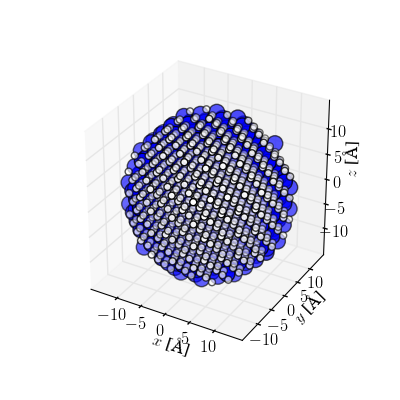
\includegraphics[width=0.45\textwidth]{img/lattice_cropped.png}}\\
% \subfloat[]{\label{fig:cropped_fixed_lattice}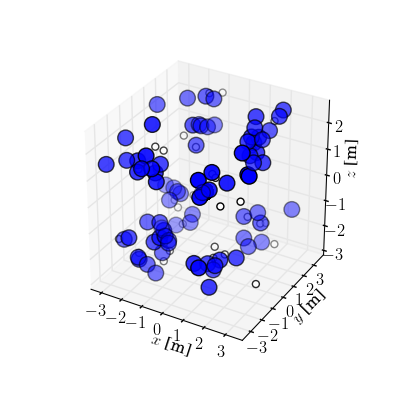
\includegraphics[width=0.45\textwidth]{img/lattice_cropped_fixed.png}}\hspace{20px}
% \subfloat[]{\label{fig:cropped_fixed_lattice_d2}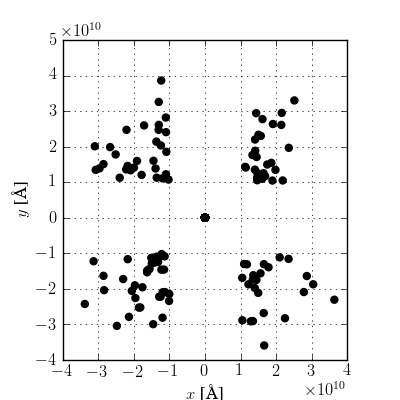
\includegraphics[width=0.4\textwidth]{img/lattice_cropped_fixed_2d.png}}
% \caption{  }
% \end{figure}


\begin{figure}[htbp]
	%\vspace{-10pt}
	\begin{center}
		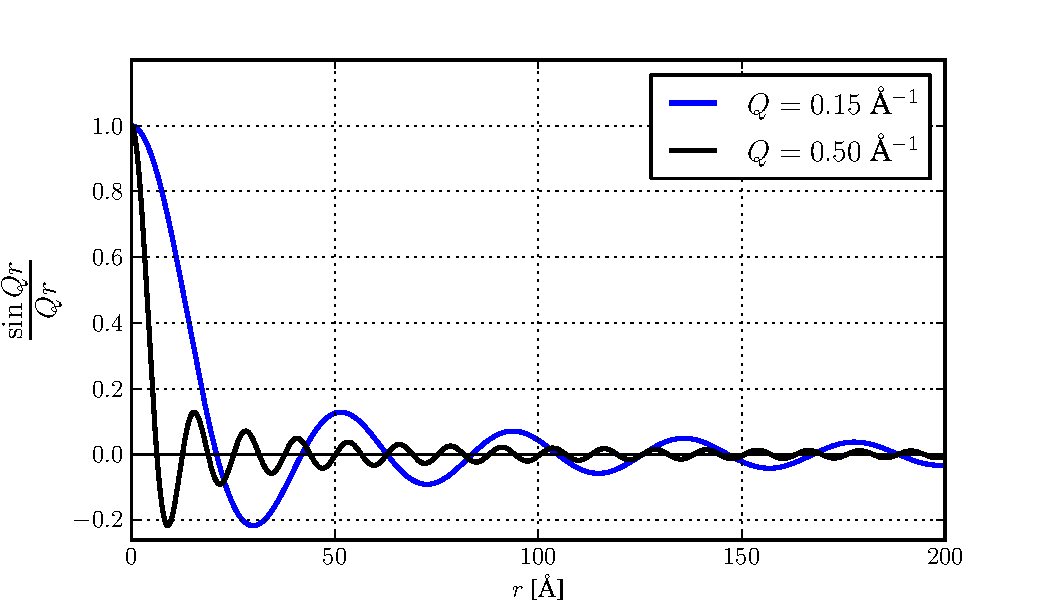
\includegraphics[width=0.85\textwidth]{img/sinc.pdf}	
	\end{center}
	%\vspace{-10pt}
	\caption{The trend of the $\operatorname{sinc}$ function in \cref{eq:inner_calc} is that it has a declining amplitude for increasingly large $r$. As a consequence, the far-away atoms that are added to the atomic arrays to make them fit the NDRange will not give any significant errors.\label{fig:sinc}}
\end{figure}




\indent After the arrays containing particle position data have been finalized they are loaded into  global memory of the GPU device. The problem is then divided into as many instances as required by~\cref{eq:i_sum_symm} to factor out the atomic form factors.  Next, the GPU calculates the contributions to $I(Q)$ tile by tile until the problem has been solved, at which time the result can be stored to a file or plotted as shown in~\cref{fig:diffractogram_random}. 


\begin{figure}[htbp]
	%\vspace{-10pt}
	\begin{center}
		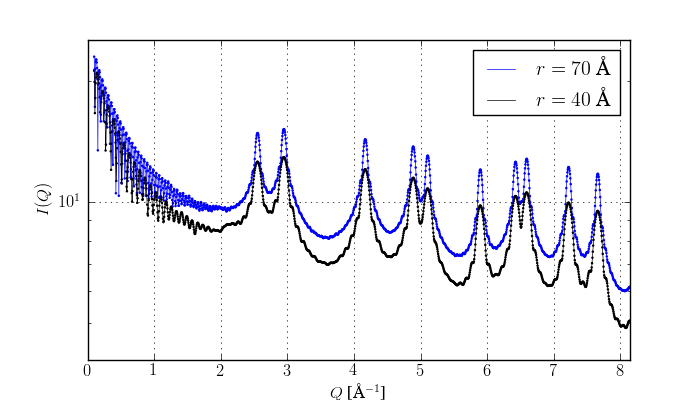
\includegraphics[width=0.85\textwidth]{img/diffractogram_random.png}	
	\end{center}
	%\vspace{-10pt}
	\caption{The result $I(Q)$ for spherical~\chem{CoO} particles with radius $40$ and $70$ \AA~(close to~\num{1.4e4} and~\num{1.5e5} atoms, respectively). The plots have $1456$ $Q$-points. The calculations for the largest particle took 8 minutes and 31 seconds to compute, and the calculations for the smallest particle took 18 seconds. The section up to $Q = 2$ [\AA] gives the Small Angle X-ray Scattering (SAXS), and the rest constitutes the Wide Angle X-ray Scattering (WAXS). The peaks in the WAXS region correspond to inter-atomic distances, while the SAXS region corresponds to larger distances such as particle size and separation. The largest particle has sharper and more intense reflections due to a higher degree of long-range order (although "long" in this context still is on the nano-scale). \label{fig:diffractogram_random}}
\end{figure}

\begin{figure}[htbp]
	%\vspace{-10pt}
	\begin{center}
		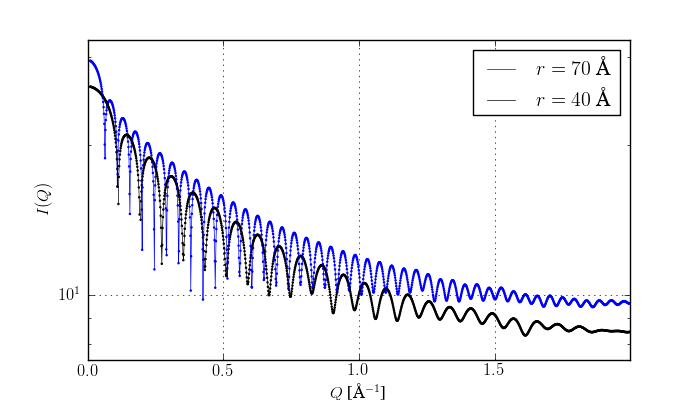
\includegraphics[width=0.85\textwidth]{img/diffractogram_random2.png}	
	\end{center}
	%\vspace{-10pt}
	\caption{Small Angle X-ray Scattering (SAXS) for spherical~\chem{CoO} particles with radius $40$ and $70$ \AA. The plots correspond to the form factor squared, $|f({\mathbf Q})|^{2}$, of spheres  with the same radii as the particles and where $\rho(\mathbf{r}) =~constant$  (cf.~\cref{eq:atomic_form_factor}).\label{fig:diffractogram_random2}}
\end{figure}

% RESULTS & DISCUSSION
\chapter{Results and Discussion\label{sec:results_discussion}}
The previous chapters lead to the description of two kernels, capable of calculating X-ray scattering for relatively complex particles. The following discussion focuses on the performance and precision of these algorithms, and how well they can be expected to scale for future graphics cards. 

\indent It is important to note that the tests performed in this chapter were done using a specific graphics card, and that any results presented here may differ from other GPUs and systems. The test system comprised a NVIDIA GTX 470 GPU combined with a $2.8$ GHz Intel Xeon X3460 CPU, both of which are in the same price range. The GTX 470 has $48$ KB of local memory and $32$ K 32-bit registers for each of its 14 compute units. All performance measurements have been done using a grid containing $2\times14N_{Q,wg}$ work groups, cf.~\cref{sec:NDRange}.

\section{Performance\label{sec:results_perf}}
Getting appreciable performance on graphics cards is often more involved than just following the guidelines in~\cref{sec:performance}. There are some parameters that affect performance in ways that are hard to predict, such as the number of work items per work group, $N_{wi}$, and the amount of shared memory and registers allocated to each work group. These variables are closely tied to the algorithm parameters  discussed in this text, and finding a good balance between them has proven to be crucial. \Cref{tab:params} lists the significant input variables and the consequences of changing them.
 % due to taking up more registers that are allocated per work item.\\
\begin{table}[htbp]
\caption{Comparison of the parameters of the rectangle and triangle algorithms that affect performance, cf.~\cref{sec:algo}.  \label{tab:params}}

\begin{center}
\scalebox{0.85}{
	
	\begin{tabular}{p{2.1cm}p{2.6cm}p{9.3cm}}
		\textbf{Input}\\ \textbf{parameter} & \textbf{Resource} & \textbf{Effect of incrementing}\\
		\toprule[2px]			
		$N_{wi}$ & Registers, local memory & Sets the minimum size of {\tt s\_flush\_V} and {\tt s\_flush\_H}. May reduce the number of resident work groups on a compute unit.\\
		\hline
		Size of\\ {\tt s\_flush\_V} & Registers, local memory & Less redundant memory transfers but taxes local memory. Unrolls by a factor $K$ at the cost of additional register usage, cf.~\cref{sec:unroll,sec:algo}. Increases arithmetic density.\\
		\hline
		Size of\\ {\tt s\_flush\_H} & Local memory & Increasing does not contribute to fewer redundant memory transfers. Consumes more local memory. \\
		\hline
		$N_{Q,wg}$ & Registers, local memory & Unrolls by a factor $N_{Q,wg}$ at the cost of registers and local memory. Increases arithmetic density.\\
		\bottomrule[2px]	
	\end{tabular}
}	
\end{center}
\end{table}

\indent As shown in~\cref{fig:s_flush_H}, increasing the size of {\tt s\_flush\_H} results in performance losses. The most prominent effect of increasing the size of {\tt s\_flush\_H}  beyond $N_{wi}$ is increased use of local memory, which it is better to allocate for other purposes. It also decreases the required number of tiles for each work group, and thus the number of parallel reductions\footnote{Recall that several arrays are summed using parallel reduction after processing each tile.} that  take place. However, the parallel reductions are carried out relatively few times in comparison to other operations, and they are unlikely to limit the performance of these kernels. This leads to the conclusion that the size of {\tt s\_flush\_H} should be set to its minimum value, i.e.\ $N_{wi}$  to avoid excessive use of local memory.

\begin{figure}[htbp]
	%\vspace{-10pt}
	\begin{center}
		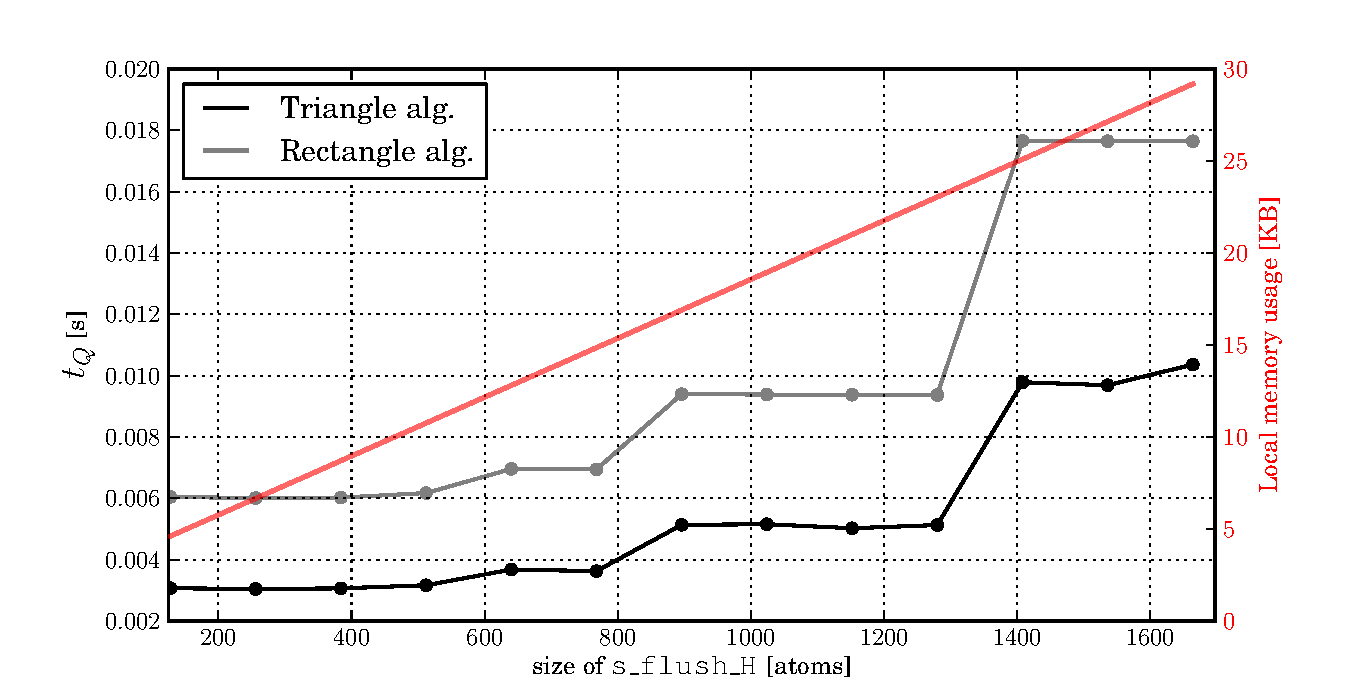
\includegraphics[width=\textwidth]{img/40_sflushH.pdf}	
	\end{center}
	%\vspace{-10pt}
	\caption{Increasing the size of {\tt s\_flush\_H} eventually resulted in performance losses. The plot shows how much time  it took to calculate ~\cref{eq:rectangle_inner,eq:square_inner} for {\it one} value of $Q$, denoted by $t_{Q}$,  as a function of the size of {\tt s\_flush\_H}.  All other parameters were set to their default (i.e.\ minimal) values. The behavior can be explained by excessive use of local memory. Note the sudden decrease in performance (and increase in $t_{Q}$) where the usage of local memory  exceeds half of the available amount, i.e.\ 24 of 48 KB. At this point it is only be possible for the compute units to host a single concurrent work group, meaning that other work groups cannot be serviced while waiting for memory fences (cf.~\cref{sec:NDRange}). \label{fig:s_flush_H}}
\end{figure}

There are three remaining parameters: $N_{Q,wg}$ and the size of {\tt s\_flush\_V} can be expected to have some positive effects on performance since they both contribute to higher arithmetic density and unrolling, cf.~\cref{sec:algo}. Besides, it is encouraged to experiment with different work group sizes, $N_{wi}$~\cite{opencl.programming}. However, the size should be a power of two due to the parallel reduction (cf.~\cref{sec:parallel_reduction}). Furthermore, the maximum number of work items per work group for the NVIDIA GTX 470 is $1024$, and the warp size is $32$. Given these constraints, the number of work items per work group should be either 32, 64, 128, 256, 512, or 1024. 
%$N_{wi}= 32$ was abandoned  due to a maximum of eight simultaneous work groups per compute unit for the device, which would limit the number of concurrent warps and thus the occupancy.
The other two parameters\footnote{The meanings of $N_{Q,wg}$ and $K$  are clarified in~\cref{tab:params}.}, $N_{Q,wg}$ and $K$, can take any values as long as there is enough local memory and available registers to launch at least one work group. 

\indent The performance for all possible combinations of the three parameters have been measured using a script that runs through any specified ranges of the input variables. A graphical representation of some of the results is shown in~\cref{fig:optimize}. \Cref{tab:combinations} shows the combinations of parameters that achieved best performance for each of the work group sizes. 


\begin{figure}[htbp]
	%\vspace{-10pt}
	\begin{center}
		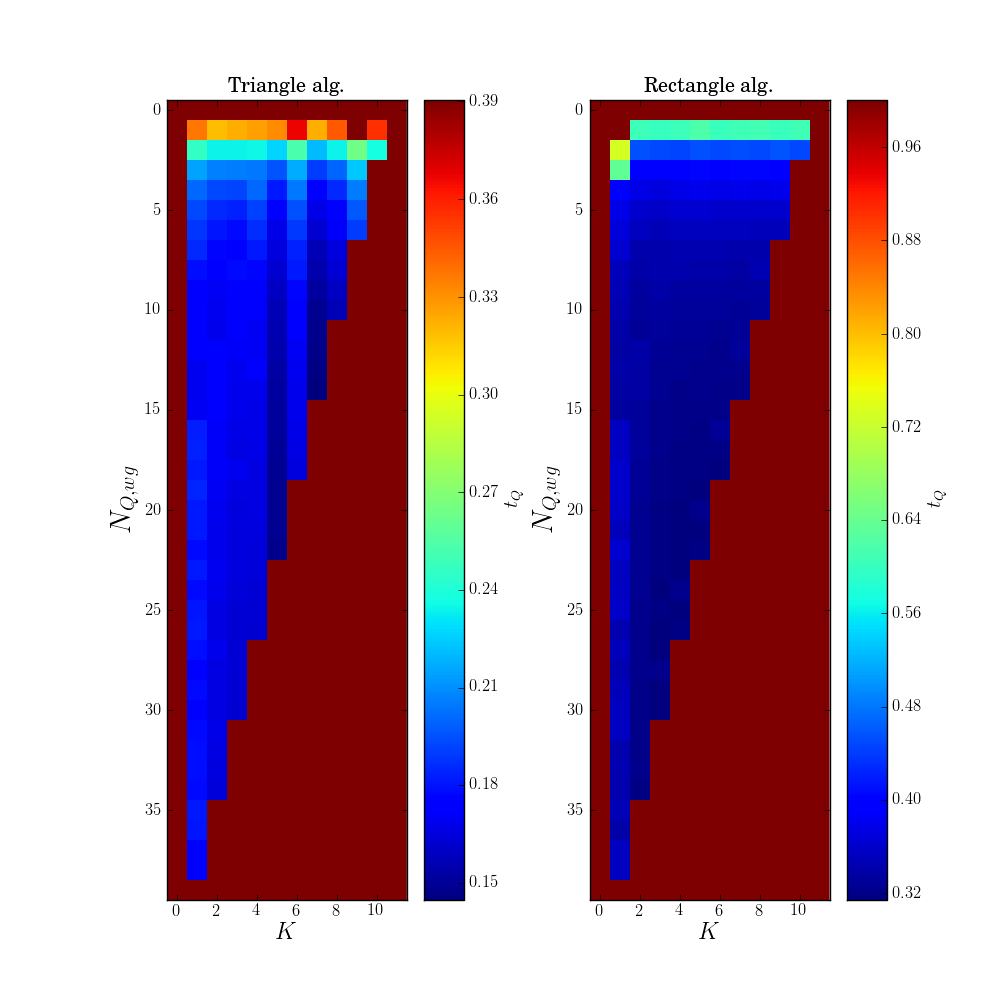
\includegraphics[width=\textwidth]{img/256_9216_OPTIMIZE.png}	
	\end{center}
	%\vspace{-10pt}
	\caption{With a work group size of 256 the optimization parameters can take a multitude of different combinations.  Recall from~\cref{sec:algo} that $K$ is an unrolling factor that is equal to the size of {\tt s\_flush\_V} divided by $N_{wi}$. $t_{Q}$ is  the time it takes to calculate a single instance of~\cref{eq:rectangle_inner} or~\cref{eq:square_inner} for one value of $Q$. $t_{Q}$ has only been measured for those combinations of the parameters that cause a work group to use less than $48$~KB of local memory, since exceeding the local memory limit results in an error.   \label{fig:optimize}}
\end{figure}


\begin{table}[htbp]
\caption{Comparison of the optimization parameters that resulted in the best performance. $t_{Q}$ is  the time it takes to calculate a single instance of~\cref{eq:square_inner} or~\cref{eq:rectangle_inner} for one value of $Q$.  The results have been measured for $N \approx \num{5e4}$ atoms and normalized to match that of a particle with exactly $N = \num{50.000}$ atoms.
$R$ denotes the ratio between the time spent by the rectangle and the triangle algorithms. One combination produced an error and has been marked with N/A.\label{tab:combinations}}
\begin{center}
\scalebox{0.70}{

	\begin{tabular}{p{3.5cm}p{1cm}p{1cm}p{0.5cm}p{3cm}p{1cm}p{1cm}p{0.5cm}p{3cm}p{1.0cm}}
		 & \multicolumn{4}{c}{\textbf{Triangle algorithm}}& \multicolumn{4}{c}{\textbf{Rectangle algorithm}}\\
		\hline
		 \textbf{Size of work group} & $t_{Q}$~[ms] & $N_{Q,wg}$ & $K$ & Local Mem. [KB] &$t_{Q}$~[ms]& $N_{Q,wg}$ & $K$ & Local Mem. [KB] & $R$\\
		\toprule[2px]			
		1024  &  \multicolumn{4}{c}{N/A}  &  99.17  &  3  &  1  &  45.068  &  N/A \\

		\hline
		512  &  42.07  &  7  &  3  &  47.132  &  80.92  &  11  &  2  &  47.148  &  1.92 \\

		\hline
		256  &  39.28  &  26  &  4  &  47.208  &  78.53  &  23  &  4  &  44.124  &  2.00 \\

		\hline
		128  &  40.08  &  18  &  6  &  23.624  &  79.06  &  31  &  3  &  24.188  &  1.97 \\
		\hline
		64  &  57.50  &  26  &  12  &  20.072  &  109.98  &  51  &  6  &  20.428  &  1.91 \\

		\hline
		32  &  113.11  &  40  &  18  &  15.008  &  209.16  &  16  &  5  &  5.184  &  1.84921876661 \\


		\bottomrule[2px]		
	\end{tabular}
}	
\end{center}
\end{table}


\indent Even though the local memory spent per $Q$-value is lower for small $N_{wi}$, the best times were achieved with $N_{wi} = 256$ and $K = 4$ for both algorithms, and with $N_{Q,wg} = 26$ and $23$ for the triangle and the rectangle algorithms, respectively. Note that the triangle algorithm spends approximately half the time of the rectangle algorithm, which it should. Also, there is a tendency for the work groups to occupy either all or half of the local memory. Kernels that use only half can launch two concurrent work groups per compute unit, which is beneficial due to memory fences that are used in the algorithms (cf.~\cref{sec:NDRange}). 



\indent The optimization routines were carried out for $N \approx \num{5e4}$. A spot check for $N \approx \num{1e5}$ that was carried out for $N_{wi} = 256$ yielded the same ratios between the results as for $N \approx \num{5e4}$. Furthermore, in terms of performance, the only significant difference between varying $N$ is the number of tiles that need to be calculated for each work group. Based on these findings the optimization routines for $N \approx \num{5e4}$ have been assumed to be valid for considerably greater values of $N$.

\indent \Cref{fig:optimize} needs some further explanation. The dark red areas represent those combinations of $K$ and $N_{Q,wg}$ that exceed the local memory limit of $48$ KB or fall outside of the chosen parameter ranges. Furthermore, it is a trend that the performance increases for high $N_{Q,wg}K$, i.e. where the most of the local memory is utilized. It is therefore tempting to conclude that local memory is the major bottleneck. However, investigation of the kernel source code for the best-performing combinations of $K$ and $N_{Q,wg}$ revealed register usage close to the maximum limit of 32 KB, with the complete unrolling (cf.~\cref{sec:algo}) requiring more than $N_{wi}N_{Q,wg}K$ registers per work group. Moreover, Gelisio et al.~\cite{ISI:000277392600034} report calculating $I(Q)$ in batches of $24$ $Q$-steps on a NVIDIA GTX 285 graphics card with only $16$ KB of local memory per compute unit, and go on to suggest that local memory is an important performance limiter for their calculations. Better control of register usage should therefore be implemented for the triangle and rectangle algorithms to investigate whether excessive register usage is a limiting factor\footnote{NVIDIA's Visual Profiler, a kernel benchmark program, does in fact say that registers are limiting the occupancy.} for high $K$ and $N_{Q,wg}$. This could be realized by use of separate unrolling factors for these parameters to prevent potentially excessive register usage  while still increasing the arithmetic density  (cf.~\cref{sec:unroll}). The resulting algorithm should initially be run with no unrolling at all to find the optimal values of $K$ and $N_{Q,wg}$, and then optimized for the two  unrolling factors. 

\indent \Cref{fig:theshit} shows performance comparisons of the initial and the optimized GPU algorithms. A plot for a CPU based double precision equivalent of the triangle algorithm written in C has also been included. This CPU code was programmed for performance, calculating $N_{Q}$ $Q$-steps for each new $r_{ij}$, but has not been as carefully constructed as the GPU algorithms. The optimized triangle algorithm is three orders of magnitude faster than the CPU code, and it is uncertain whether this  performance gap can be attributed to insufficient optimization of the CPU code alone. Moreover,the optimized GPU codes are about two to three times as fast as the initial, or default, algorithms where $K = N_{Q,wg} = 1$. 


%The number of resident warps, and thus the occupancy (cf.~\cref{sec:NDRange}), is inversely proportional to number of registers assigned to each .  
%-this could be a good place to include various plots.
\begin{figure}[htbp]
	%\vspace{-10pt}
	\begin{center}
		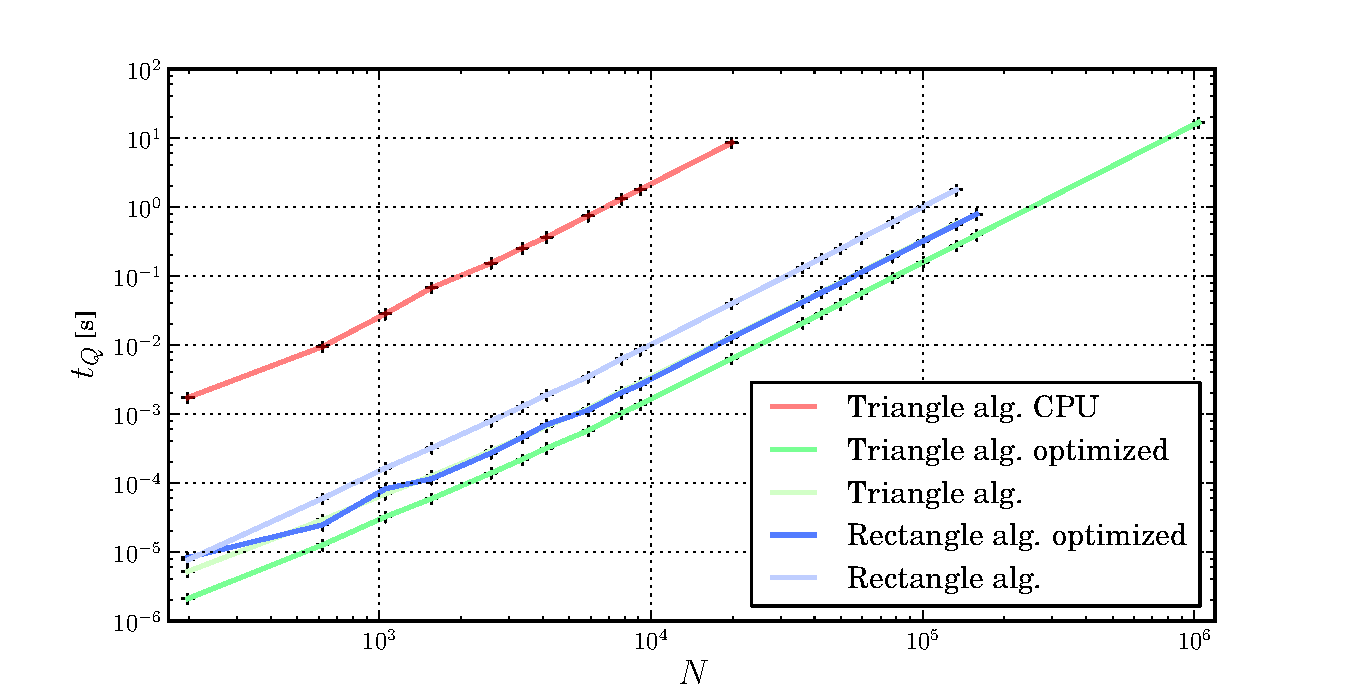
\includegraphics[width=\textwidth]{img/_N_t_supermegaplot.pdf}	
	\end{center}
	%\vspace{-10pt}
	\caption{$t_{Q}$ as a function of $N$ for the rectangle and triangle algorithms before and after optimizing $N_{Q,wg}$, $K$, and $N_{wi}$. $N$ excludes atoms that were added after the crop, cf.~\cref{sec:framework}. The optimized triangle algorithm achieves more than a $1000\times$ speedup over corresponding CPU algorithm. Furthermore, it is over twice as fast as the default algorithm with $K = N_{Q,wg} = 1$. The scaling factor is $2$ for all alogrithms. The optimized rectangle algorithm overlaps the plot for the default version of the triangle algorithm to some extent.  \label{fig:theshit}}
\end{figure}


\indent In order to further improve performance, the algorithm could be modified to ignore calculations involving padding atoms, thus eliminating the need for the framework routine that places these atoms around the lattice. The extra logic needed for this would influence the performance gain. There might also be a marginal benefit in precision.

\indent On a final note, the efficiency of the Python framework has proven sufficient for the purpose of conducting performance tests, and generally takes only a small fraction of the time of the subsequent X-ray simulation.


\section{Precision}
%-Precision
%What measures ahve been taken so as to minimize precision losses
%Validity of native_sin and divide
In order to measure the accumulation of single precision errors in the triangle algorithm a plot of $I(Q)$ for $N = 13700$ atoms\footnote{The \chem{Co} atoms of an \chem{CoO} lattice were used.} was compared to a corresponding plot generated by a double precision CPU code implemented in C. \Cref{fig:single_double} shows the standard deviation of the difference between the two data sets, and it is assumed that the double precision  implementation has substantially higher accuracy. The double precision code has been optimized with respect to precision to make this assumption more valid.  The standard deviation gives a relative error of $\num{5e-5}$ for the small feature at $Q \approx 5.8$ \AA~and a relative error of  $\num{5e-6}$ for the largest peak at $Q \approx 2.5$ \AA. Note that the CPU algorithm does not rely on padding atoms to meet NDRange requirements, and, moreover, that simulations for larger values of $N$ did not increase the relative error.

\indent Several factors limit the intensity resolution of real world diffraction experiments and introduce errors. Examples of such factors are instrument resolution and  correction factors. Measurements where the error is below a few percent are often considered to be excellent. The error implied by~\cref{fig:single_double} is therefore relatively low in comparison. The purpose for generating simulated X-ray diffraction models is to compare the output data to real world results, and if there is already an error of a few percent, an additional relative error of $\num{5e-5}$ is not going to make much difference.     

\begin{figure}[htbp]
	%\vspace{-10pt}
	\begin{center}
		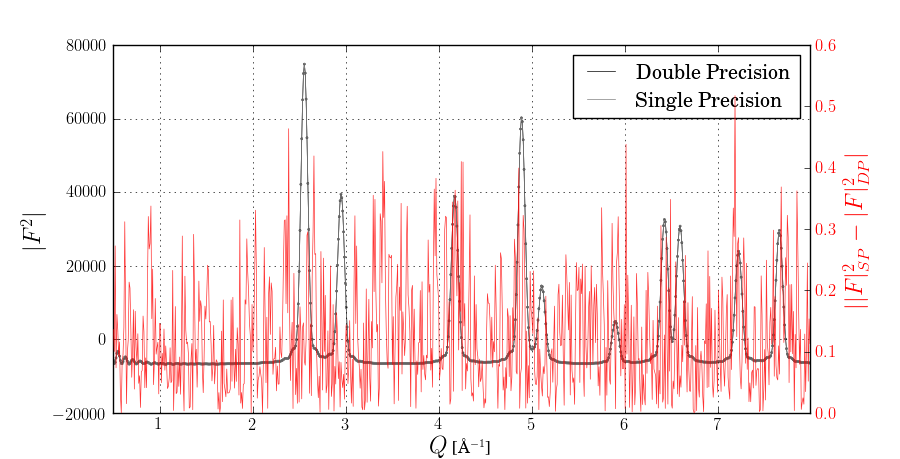
\includegraphics[width=1\textwidth]{img/13700_single_double.png}	
	\end{center}
	%\vspace{-10pt}
	\caption{The standard deviation between the triangle algorithm and a precision optimized CPU code for a particle of $N = \num{1.3e4}$ atoms. The standard deviation gives a relative error of $\num{5e-5}$ for the small feature at $Q \approx 5.8$ \AA~and a relative error of  $\num{5e-6}$ for the largest peak at $Q \approx 2.5$ \AA\label{fig:single_double}}
\end{figure}

The GPU algorithms replace the $\sin$ function and the division operator in \cref{eq:inner_calc} by native functions. The precision of {\tt native\_sin} is shown in~\cref{fig:native_functions_STD}. According to the data, the simulations presented in this report do not introduce relative errors greater than $0.01$\% ($r_{ij} < 500$ \AA). However, for large values of $Qr_{ij}$ the native function should be substituted by the more accurate and much more computationally heavy $\sin$ function. Finally, the GTX 470's {\tt native\_divide} function has the same accuracy as the normal implementation. 




\section{Scaling}
\Cref{sec:NDRange} states that a kernel invocation should result in thousands of work groups in order to scale for multiple  generations of future  GPU devices. Given that that the number of work groups is $N_{Q}/N_{Q,wg}$, this is only the case for either high values of $N_{Q}$ or low values of $N_{Q,wg}$. For the triangle and rectangle algorithms discussed in this report the most efficient combinations of parameters use $N_{Q,wg} = 26$ and $23$, respectively. However, the GTX 470 is one of the first architectures that allows for multiple kernels to run simultaneously on one device. \Cref{eq:square_inner,eq:rectangle_inner} can therefore be split into as many sub-equations as necessary for a given system and invoked simultaneously as multiple kernels to get the desired amount of work groups.  There are in addition other ways to split the workload over more work groups, such as splitting the work done by each work group {\it within} the kernel rather than over multiple kernels. In the latter approach each work group would process a given number of tiles to match any need.
%Show own   N_{Q,wg} in plots!

% CONCLUSIONS
\chapter{Conclusion and Further Work}
A program that calculates the powder diffraction pattern of nano-sized particles has been written to run in single precision on GPUs using the OpenCL API. The performance  and precision of this software has been compared to a CPU based program running in double precision. Additionally, several optimization techniques have been employed to better utilize the hardware resources present on the graphics card.

\indent Findings include a significant speedup from the CPU based double precision algorithm to the optimized GPU based single precision algorithm at a tolerable  precision loss. Moreover, there was a $2$ - $3\times$ performance gain when optimizing the GPU algorithms with respect to usage of registers and fast, on-chip local memory. It was also argued that excessive register usage could be a key performance limiting factor, as well as a limited local memory cache as suggested by  Gelisio et al.


\indent The purpose of simulating powder diffraction patterns is of course to do comparative analyses with experimental results, and future work could therefore include writing of GPU-accelerated software for such purposes, for example by matching experimental data to previously generated diffraction patterns. 

\indent Future work could also include rewriting the GPU algorithms to see if even better performance can be achieved by increasing control over the loop unrolling and thereby use fewer registers. Additionally, the algorithm can be modified to ignore calculations involving padding atoms so as to slightly improve both performance and precision. Finally, the algorithm can be implemented to run on systems comprising multiple GPUs.


%Implement controlled unrolling.
%Ray Tracing, DFT, FFT (and other embarrassingly parallel problems)
%Make frequency of parallel reductions an input parameter, and give the option of summing a results array in double precision.
%Conclusion
%-Make model of nearest neighbours
%-Discuss future works
%-Multiple gpu
%-Improving Precision
\addtolength{\textwidth}{-5cm} %next four lines are margin control
\addtolength{\hoffset}{1.5cm}
\addtolength{\textheight}{-4cm}
\addtolength{\voffset}{2cm}


\newpage
% APPENDIX
%\begin{subappendices}
\appendix 
\chapter{Calculating Theoretical Performance}
\section{FLOPS}
\label{app:FLOPS}
Floating Point Operations Per Second (FLOPS) is a commonly used measure of the theoretical performance of a system or device. However, there are many other factors that influence actual instruction performance. This paragraph describes how to calculate FLOPS for a General processing Unit (GPU).


\indent  Modern GPUs are often measured by the number of Fused Multiply Add (FMA)  instructions they can calculate per second times two. The FMA instruction calculates an expression of the type $ab +c$, and is therefore both a multiplication operation and an addition operation in one. The performance in FLOPS is then given by 

\begin{equation}
	2\times(number~of~cores)\times(shader~frequency) ,
\end{equation}

\noindent where  $shader~frequency$ corresponds to the frequency of each core (i.e.\ processing element). For example, the NVIDIA GTX 470 has 14 compute units with 32 cores each running at a frequency of 1.215 GHz, resulting in a performance of $2\times14\times32\times1.215 \mbox{ GFLOPS }= 1088.64 \mbox{ GFLOPS }$.
%The Radeon HD 5870 has 1600 usable stream cores, while the Radeon HD 5850 has 1,440 usable stream cores, as 160 out of the 1,600 total cores are disabled during product binning which detects potentially defective areas of the chip
%Why are these benchmarks only theoretical? Why do they not have as much importance as one would think? (Drivers and much more)

%FLOPS can be ADD/MUL/DIVIDE/MUL+ADD. MUL+ADD considered as two FLOPs?

%FLOPS is, as the name implies FLoating point OPerations per Second, exactly what constitutes a FLOP might vary by CPU. (Some CPU's can perform addition and multiplication as one operation, others can't, for example). That means that as a performance measure, it is fairly close to the hardware, which means that 1) you have to know your hardware to compute the ideal FLOPS on the given architecture, and you have to know your algorithm and implementation to figure out how many floating point ops it actually consists of.

%In any case, it's a useful tool for examining how well you utilize the CPU. If you know the CPU's theoretical peak performance in FLOPS, you can work out how efficiently you use the CPU's floating point units, which are often one of the hard to utilize efficiently. A program which runs 30% of the FLOPS the CPU is capable of, has room for optimization. One which runs at 70% is probably not going to get much more efficient unless you change the basic algorithm. For math-heavy algorithms like yours, that is pretty much the standard way to measure performance. You could simply measure how long a program takes to run, but that varies wildly depending on CPU. But if your program has a 50% CPU utilization (relative to the peak FLOPS count), that is a somewhat more constant value (it'll still vary between radically different CPU architectures, but it's a lot more consistent than execution time).

\section{Memory Bandwidth}
\label{app:MBW}
Memory Bandwidth (MBW) is the rate at which data can be read from or stored into a semiconductor memory by a processor. For graphics cards, memory bandwidth is associated with the speed at which data is transferred between global memory and the cores (i.e.\ processing elements). The theoretical peak memory bandwidth for a graphics card is given by

\begin{equation}
	(memory~frequency)\times(memory~bus~width) ,
\end{equation}


\noindent where $memory~bus~width$ denotes the amount of data transferred per global memory clock cycle. For example, the global memory of the GTX 470 operates at a frequency of $3.348$ GHz and has a $320$-bit $= 40$ bytes bus width, and therefore peaks at $3.348\times40 \mbox{GB/s} = 133.92 \mbox{GB/s}$.

\indent  Calculating  the peak theoretical MBW and comparing it to the actual memory transfer rate for an algorithm (i.e.\ a kernel) is helpful to see if memory is limiting performance. 
\newpage
%\section{Python code}
%\subsection{run.py}
%\lstset{language=Python,caption={},label=run}
%\lstinputlisting[language=Python, style=my_Python]{python_source/run.py}
%\newpage

%\subsection{structures\_library.py}
%\lstset{language=Python,caption={},label=library}
%\lstinputlisting[language=Python, style=my_Python]{python_source/structures_library.py}
%\newpage

%\subsection{debye\_kernels\_v1\_0.py}
%\lstset{language=Python,caption={},label=kernel}
%\lstinputlisting[language=Python, style=my_Python]{python_source/debye_kernels_v1_0.py}
%\newpage

%\subsection{unroll.py}
%\lstset{language=Python,caption={},label=unroll}
%\lstinputlisting[language=Python, style=my_Python]{python_source/unroll.py}
%\newpage

%\subsection{structure\_finetune.py}
%\lstset{language=Python,caption={},label=finetune}
%\lstinputlisting[language=Python, style=my_Python]{python_source/structure_finetune.py}
%\newpage

%\subsection{structure\_crop.py}
%\lstset{language=Python,caption={},label=crop}
%\lstinputlisting[language=Python, style=my_Python]{python_source/structure_crop.py}
%\newpage

%\subsection{LPG.py}
%\lstset{language=Python,caption={},label=LPG}
%\lstinputlisting[language=Python, style=my_Python]{python_source/LPG.py}
%\newpage
%\end{subappendices}

\addcontentsline{toc}{section}{{\bf References}}
\bibliographystyle{ieeetr}
\bibliography{bibfile.bib}


\end{document}
